\documentclass{article}\usepackage[]{graphicx}\usepackage[]{color}
% maxwidth is the original width if it is less than linewidth
% otherwise use linewidth (to make sure the graphics do not exceed the margin)
\makeatletter
\def\maxwidth{ %
  \ifdim\Gin@nat@width>\linewidth
    \linewidth
  \else
    \Gin@nat@width
  \fi
}
\makeatother

\definecolor{fgcolor}{rgb}{0.345, 0.345, 0.345}
\newcommand{\hlnum}[1]{\textcolor[rgb]{0.686,0.059,0.569}{#1}}%
\newcommand{\hlstr}[1]{\textcolor[rgb]{0.192,0.494,0.8}{#1}}%
\newcommand{\hlcom}[1]{\textcolor[rgb]{0.678,0.584,0.686}{\textit{#1}}}%
\newcommand{\hlopt}[1]{\textcolor[rgb]{0,0,0}{#1}}%
\newcommand{\hlstd}[1]{\textcolor[rgb]{0.345,0.345,0.345}{#1}}%
\newcommand{\hlkwa}[1]{\textcolor[rgb]{0.161,0.373,0.58}{\textbf{#1}}}%
\newcommand{\hlkwb}[1]{\textcolor[rgb]{0.69,0.353,0.396}{#1}}%
\newcommand{\hlkwc}[1]{\textcolor[rgb]{0.333,0.667,0.333}{#1}}%
\newcommand{\hlkwd}[1]{\textcolor[rgb]{0.737,0.353,0.396}{\textbf{#1}}}%
\let\hlipl\hlkwb

\usepackage{framed}
\makeatletter
\newenvironment{kframe}{%
 \def\at@end@of@kframe{}%
 \ifinner\ifhmode%
  \def\at@end@of@kframe{\end{minipage}}%
  \begin{minipage}{\columnwidth}%
 \fi\fi%
 \def\FrameCommand##1{\hskip\@totalleftmargin \hskip-\fboxsep
 \colorbox{shadecolor}{##1}\hskip-\fboxsep
     % There is no \\@totalrightmargin, so:
     \hskip-\linewidth \hskip-\@totalleftmargin \hskip\columnwidth}%
 \MakeFramed {\advance\hsize-\width
   \@totalleftmargin\z@ \linewidth\hsize
   \@setminipage}}%
 {\par\unskip\endMakeFramed%
 \at@end@of@kframe}
\makeatother

\definecolor{shadecolor}{rgb}{.97, .97, .97}
\definecolor{messagecolor}{rgb}{0, 0, 0}
\definecolor{warningcolor}{rgb}{1, 0, 1}
\definecolor{errorcolor}{rgb}{1, 0, 0}
\newenvironment{knitrout}{}{} % an empty environment to be redefined in TeX

\usepackage{alltt}
\usepackage{booktabs}
\usepackage{longtable}
\usepackage{array}
\usepackage{multirow}
\usepackage{wrapfig}
\usepackage{float}
\usepackage{colortbl}
\usepackage{pdflscape}
\usepackage{tabu}
\usepackage{threeparttable}
\usepackage{threeparttablex}
\usepackage[normalem]{ulem}
\usepackage{makecell}
\usepackage{url}
\usepackage{amsmath}
\usepackage[bottom]{footmisc}
\usepackage{Rd}
\newenvironment{Arg}{%
\begin{Rdsection}{}}{\end{Rdsection}}

\title{trajeR package\\
\medskip
\includegraphics[scale=0.4]{/mnt/Travail/These/logo/logo5.png}}
\author{Cédric NOEL - Jang SHILTZ\\
cedric.noel@univ-lorraine.fr}
\IfFileExists{upquote.sty}{\usepackage{upquote}}{}
\begin{document}
\maketitle

\tableofcontents

\newpage

\section{Introduction}
Longitudinal studies are often employed on several disciplines like finance, econometrics, psychology, sociology, biology,  ...\\

The aims of this package is to give tools to work with this situation.\\

More precisely, we consider a variable $Y$  that evolves over time.

\section{Getting started}

First, we need to install \verb|trajeR| package.
\begin{knitrout}
\definecolor{shadecolor}{rgb}{0.969, 0.969, 0.969}\color{fgcolor}\begin{kframe}
\begin{alltt}
\hlkwd{library}\hlstd{(trajeR)}
\end{alltt}


{\ttfamily\noindent\itshape\color{messagecolor}{\#\# Loading required package: MASS}}

{\ttfamily\noindent\itshape\color{messagecolor}{\#\# Loading required package: minpack.lm}}\end{kframe}
\end{knitrout}

The main function is named \verb|trajeR|. It fit the model and find parameters to a given degre of polynomial shape. It syntax is

\begin{knitrout}
\definecolor{shadecolor}{rgb}{0.969, 0.969, 0.969}\color{fgcolor}\begin{kframe}
\begin{alltt}
\hlkwd{trajeR}\hlstd{(Y, A,} \hlkwc{X} \hlstd{=} \hlkwa{NULL}\hlstd{,} \hlkwc{TCOV} \hlstd{=} \hlkwa{NULL}\hlstd{, ng, degre,} \hlkwc{degre.nu} \hlstd{=} \hlnum{0}\hlstd{, Model,}
       \hlkwc{Method} \hlstd{=} \hlstr{"L"}\hlstd{,} \hlkwc{ssigma} \hlstd{=} \hlnum{FALSE}\hlstd{,} \hlkwc{ymax} \hlstd{=} \hlkwd{max}\hlstd{(Y)} \hlopt{+} \hlnum{1}\hlstd{,} \hlkwc{ymin} \hlstd{=} \hlkwd{min}\hlstd{(Y)} \hlopt{-} \hlnum{1}\hlstd{,}
       \hlkwc{hessian} \hlstd{=} \hlnum{TRUE}\hlstd{,} \hlkwc{itermax} \hlstd{=} \hlnum{100}\hlstd{,} \hlkwc{paraminit} \hlstd{=} \hlkwa{NULL}\hlstd{,}
       \hlkwc{fct} \hlstd{=} \hlkwa{NULL}\hlstd{,} \hlkwc{diffct} \hlstd{=} \hlkwa{NULL}\hlstd{,} \hlkwc{nbvar} \hlstd{=} \hlkwa{NULL}\hlstd{)}
\end{alltt}
\end{kframe}
\end{knitrout}

\begin{Arguments}
	\begin{ldescription}
		\item[\code{Y}] a matrix containing the variables in the model.

		\item[\code{A}] a matrix containing the time variable data.

		\item[\code{TCOV}] an optionnal matrix containing the time covariate that influence the trajectory themselve.
		By default its value is NULL.

		\item[\code{ng}] integer. The number of group.

		\item[\code{degre}] vector of integer. The degre of every ploynomial function.

		\item[\code{degre.nu}] vecor of integer. The degre of all Poisson part for a ZIP model.

		\item[\code{Model}] the model used. The value are LOGIT for a Logit Mixture model,
		CNORM for a Censored Normal Mixture Model or ZIP for Zero Inflated Poisson Mixture model.

		\item[\code{Method}] determine the method used for find the paramters of the model.
		The value are L for the Maximum Likelihiood Estimation, EM for Expectation Maximization method
		with quasi newton method inside, EMIWRLS for Expectation Maximization method with Iterative
		Weighted ??

		\item[\code{ssigma}] logical. By default its value is FALSE. For the CNORM model,
		indicate if we want the same sigma for all nomrmal density function.

		\item[\code{ymax}] real. For the CNORM model, indicate the maximum value of the data. It oncerne only the model
		with censored data. By default its value is the maximum value of the data plus 1.

		\item[\code{ymin}] real. For the CNORM model, indicate the minimum value of the data. It oncerne only the model
		with censored data. By default its value is the maximum value of the data minus 1.

		\item[\code{hessian}] logical. Indicate if we want calculate the hessian matrix. Default is FALSE.
		If the method use is Likelihood, the hessian is calculated by inversing the Information's Fisher Matrix.
		To avoid numerically singular matrix we find the pseudo inverse matrix by using the ginv function int he package MASS.
		If the method is EM or EMIWRLS, the hessian is calculted by using Louis method.

		\item[\code{itermax}] integer. Indicate the maximal number of iteration for optim function or for the EM algorithm.

		\item[\code{paraminit}] vector. The vector of initial parameters. By default trajeR calculate the initial value
		based of the range or the standrad deviation.

		\item[\code{fct}] a function. The definition of the function  f in the definition in nonlinear model.

    \item[\code{diffct}] a function. The differential of the function f in the nonlinear model.

    \item[\code{nbvar}] integer. The number of variable in the nonlinear model.

		\item[\code{X}] an optionnal matrix that modifie the probabilty of belong to group. By default its value is a mtrix
		with one column  with value 1.
	\end{ldescription}
\end{Arguments}

\begin{Details}\relax
	Models for trajeR is, by default, a polynomial regression of the time value parameters for each groups. The number fo group is controlled by the integer \code{ng}.
	We can spcecify the degre of the polynomial shape for each groups by the vector \code{degre}.
\end{Details}
%
\begin{Value}
	return an object of class "\code{Trajectory.LOGIT}".
	The generic accessor functions \code{beta}, \code{delta}, \code{theta}, \code{sd}, \code{tab}, \code{Likelihood},
	\code{ng}, \code{model} and \code{method} extract various useful features of the value returned by \code{trajeR}.

	An object of class "\code{Trajectory.LOGIT}" is a list containing at least the following components:
\end{Value}
	\begin{Arg}
	\begin{ldescription}

		\item[\code{beta}] a vector of the parameters beta.
		\item[\code{delta}] a vector of the parameter delta. Only if we use time covariate.
		\item[\code{theta}] a vector with the paramter theta if there exist a coavriate X that modifie
		the probability or the probability of group membership.
		\item[\code{sd}] a vector of the standrad deviation of the parameters.
		\item[\code{tab}] a matrix with all the parameters and standard deviation.
		\item[\code{Likelihood}] a real with the Likelihhod obtnaied by the parameters.
		\item[\code{ng}] a integer with the number of group.
		\item[\code{model}] a string with the model used.
		\item[\code{method}] a string with the method used.

	\end{ldescription}
\end{Arg}

\section{LOGIT model}
In this section we consider a latent variable $y^*_{it}$ such that
\begin{equation}
y^*_{it} = f(a_{it}; \beta_k, \delta_k)+\epsilon_{it} =\beta_k A_{it}+\delta_k W_t+\epsilon_{it}
\end{equation}
where $\epsilon_{it}\sim \mathcal{N}\left(0;\ \sigma_k\right)$,  $A_{it}=(1,a_{it},a_{it}^2,\cdots,a_{it}^{n_\beta-1})^t $, $W_t=(w_{i1},\cdots,w_{in_\delta})^t $, $\beta_k =(\beta_{k1},\cdots, \beta_{kn_\beta})$ and $\delta_k=(\delta_{k1},\cdots,\delta_{kn_\delta}) $.\\
Under this affirmation, classically, it is assumed that the binary variable $y_{it}=1$ if $y^*_{it}>0$ and $y_{it}=0$ if $y^*_{it}\leq 0$.\\

If $\epsilon_{it}$ is assumed to be normally distributed , described the probit function.
Let $\rho_{ikt}=P(Y_{it}=1|W_i=w_i,C_i=k)$ the probability of $y_{it}=1$ given membership in group $k$.
\begin{equation}
\rho_{ikt}=\dfrac{e^{\beta_k A_{it}+\delta_k W_{it}}}{1+e^{\beta_k A_{it}+\delta_k W_{it}}}
\end{equation}

\subsection{Parameters}

\textbf{Example}\\
We use artificial data contained in the library. This are 500 longitudinal data of 0 and 1 values generate by the parameters above :
\begin{itemize}
	\item 3 groups ;
	\item probability is $\pi_1=0.22$, $\pi_2=0.44$ and $\pi_3=0.34$ ;
	\item period is 10 ;
	\item we use 3 polynomial shape
	\begin{enumerate}
		\item degre 3 and $\beta_1=(-2.266,-0.109,0.14,-0.011)$ ;
		\item degre 4 and $\beta_2=(1.291,0.811,-0.554,0.077,-0.003)$ ;
		\item degre 0 and $\beta_{3}=(-1.99243)$.
	\end{enumerate}
\end{itemize}

The data contained the time variable dependent $Y_i$ in \verb|data[,2:11]|, the time variable in \verb|data[,12:21]|, the time covariate in \verb|data[,24:33]| and a covariate that influence the belonging probabilty in \verb|data[,48:49]|.
\begin{itemize}
	\item \verb|data[,2:11]| is a matrix with 0 and 1 values.
	\item \verb|data[,12:21]| is a matrix with time 1 to 10.
	\item \verb|data[,24:33]| is a time covriate that influence the shape fo trajectory. It is a matrix with 0 and 1 value, like the presence or not of a characteristic on the individual.
	\item \verb|data[,48:49]| is a matrix with 0 and 1 value.
\end{itemize}


\begin{knitrout}
\definecolor{shadecolor}{rgb}{0.969, 0.969, 0.969}\color{fgcolor}
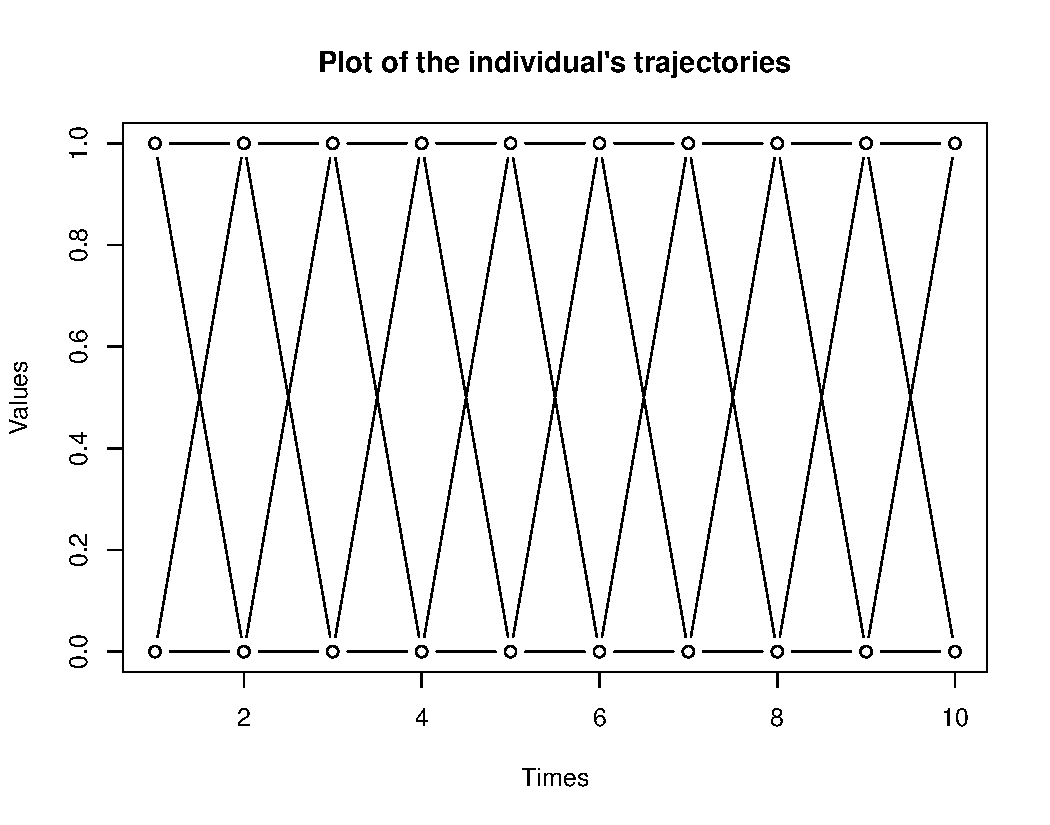
\includegraphics[width=\maxwidth]{figure/unnamed-chunk-4-1} 

\end{knitrout}
We use the each method to fit the model. For all method, we specifies the number of group of our model, ng=3, the degree of the polynomial of the shape of the trajectory. Here we choice a line parallel to abscissa axis, a cubic polynomial and a quadric polynomial. So degree is a vector $(0,3,4)$.\\
We sepcifie \verb|hessian=TRUE| to ask the calculus of the hessian matrix.\\
\verb|Itermax | is set to 300 to assure a good approximation of the parameters.\\

For the Likelihood method we call trajeR with option Method ="L".

\begin{knitrout}
\definecolor{shadecolor}{rgb}{0.969, 0.969, 0.969}\color{fgcolor}\begin{kframe}
\begin{alltt}
\hlcom{# Likelihood}
\hlstd{solL} \hlkwb{=} \hlkwd{trajeR}\hlstd{(}\hlkwc{Y} \hlstd{= data[,}\hlnum{2}\hlopt{:}\hlnum{11}\hlstd{],} \hlkwc{A} \hlstd{= data[,}\hlnum{12}\hlopt{:}\hlnum{21}\hlstd{],}
              \hlkwc{ng} \hlstd{=} \hlnum{3}\hlstd{,} \hlkwc{degre} \hlstd{=} \hlkwd{c}\hlstd{(}\hlnum{0}\hlstd{,}\hlnum{3}\hlstd{,}\hlnum{4}\hlstd{),}
              \hlkwc{Model} \hlstd{=} \hlstr{"LOGIT"}\hlstd{,} \hlkwc{Method} \hlstd{=} \hlstr{"L"}\hlstd{,} \hlkwc{hessian} \hlstd{=} \hlnum{TRUE}\hlstd{,}
              \hlkwc{itermax} \hlstd{=} \hlnum{300}\hlstd{,} \hlkwc{paraminit} \hlstd{= paraminit)}
\end{alltt}
\end{kframe}
\end{knitrout}
\begin{knitrout}
\definecolor{shadecolor}{rgb}{0.969, 0.969, 0.969}\color{fgcolor}\begin{kframe}
\begin{alltt}
\hlstd{solL}
\end{alltt}
\begin{verbatim}
## Call TrajeR with 3 groups and a 0,3,4 degrees of polynomial shape of trajectory.
## Model : Logit
## Method : Likelihood 
##  
##   group   Parameter   Estimate   Std. Error   T for H0:   Prob>|T|  
##                                                param.=0             
## --------------------------------------------------------------------
##       1   Intercept   -1.94482      0.10059   -19.33387          0  
##                                                                     
##       2   Intercept   -1.77021      0.03535   -50.07501          0  
##              Linear   -0.44043          NaN         NaN        NaN  
##           Quadratic    0.18687          NaN         NaN        NaN  
##               Cubic   -0.01232          NaN         NaN        NaN  
##                                                                     
##       3   Intercept    1.74626          NaN         NaN        NaN  
##              Linear     0.6443      0.07247     8.89028          0  
##           Quadratic    -0.5554      0.02475   -22.44466          0  
##               Cubic    0.08204      0.00195    42.07317          0  
##           Quadratic   -0.00336          NaN         NaN        NaN  
## --------------------------------------------------------------------
##       1         pi1    0.41816      0.10875     2.41645    0.01571  
##       2         pi2    0.21915      0.11423    -3.35532      8e-04  
##       3         pi3    0.36269       0.0623     1.93388    0.05318  
## --------------------------------------------------------------------
## Likelihood : -2852.749
\end{verbatim}
\end{kframe}
\end{knitrout}

For the EM method
\begin{knitrout}
\definecolor{shadecolor}{rgb}{0.969, 0.969, 0.969}\color{fgcolor}\begin{kframe}
\begin{alltt}
\hlcom{#EM}
\hlstd{solEM} \hlkwb{=} \hlkwd{trajeR}\hlstd{(}\hlkwc{Y} \hlstd{= data[,}\hlnum{2}\hlopt{:}\hlnum{11}\hlstd{],} \hlkwc{A} \hlstd{= data[,}\hlnum{12}\hlopt{:}\hlnum{21}\hlstd{],}
               \hlkwc{ng} \hlstd{=} \hlnum{3}\hlstd{,} \hlkwc{degre} \hlstd{=} \hlkwd{c}\hlstd{(}\hlnum{0}\hlstd{,}\hlnum{3}\hlstd{,}\hlnum{4}\hlstd{),}
               \hlkwc{Model} \hlstd{=} \hlstr{"LOGIT"}\hlstd{,} \hlkwc{Method} \hlstd{=} \hlstr{"EM"}\hlstd{,} \hlkwc{hessian} \hlstd{=} \hlnum{TRUE}\hlstd{,}
               \hlkwc{itermax} \hlstd{=} \hlnum{300}\hlstd{,} \hlkwc{paraminit} \hlstd{= paraminit)}
\hlcom{#EMIWRLS}
\hlstd{solEMIWRLS} \hlkwb{=} \hlkwd{trajeR}\hlstd{(}\hlkwc{Y} \hlstd{= data[,}\hlnum{2}\hlopt{:}\hlnum{11}\hlstd{],} \hlkwc{A} \hlstd{= data[,}\hlnum{12}\hlopt{:}\hlnum{21}\hlstd{],}
                    \hlkwc{ng} \hlstd{=} \hlnum{3}\hlstd{,} \hlkwc{degre}\hlstd{=}\hlkwd{c}\hlstd{(}\hlnum{0}\hlstd{,}\hlnum{3}\hlstd{,}\hlnum{4}\hlstd{),}
                    \hlkwc{Model} \hlstd{=} \hlstr{"LOGIT"}\hlstd{,} \hlkwc{Method} \hlstd{=} \hlstr{"EMIWRLS"}\hlstd{,} \hlkwc{hessian} \hlstd{=} \hlnum{TRUE}\hlstd{,}
                    \hlkwc{itermax} \hlstd{=} \hlnum{300}\hlstd{,} \hlkwc{paraminit} \hlstd{= paraminit)}
\end{alltt}
\end{kframe}
\end{knitrout}


\begin{knitrout}
\definecolor{shadecolor}{rgb}{0.969, 0.969, 0.969}\color{fgcolor}\begin{kframe}
\begin{alltt}
\hlstd{solEM}
\end{alltt}
\begin{verbatim}
## Call TrajeR with 3 groups and a 0,3,4 degrees of polynomial shape of trajectory.
## Model : Logit
## Method : Expectation-maximization 
##  
##   group   Parameter   Estimate   Std. Error   T for H0:   Prob>|T|  
##                                                param.=0             
## --------------------------------------------------------------------
##       1   Intercept   -1.94758      0.08026   -24.26591          0  
##                                                                     
##       2   Intercept   -1.20632       0.5722    -2.10821    0.03506  
##              Linear    -0.6683        0.346    -1.93153    0.05347  
##           Quadratic    0.21428      0.06328      3.3861    0.00071  
##               Cubic   -0.01332      0.00351    -3.79284    0.00015  
##                                                                     
##       3   Intercept    1.77994      0.30856     5.76856          0  
##              Linear    0.74524      0.36981     2.01519    0.04394  
##           Quadratic   -0.59753      0.13358    -4.47325      1e-05  
##               Cubic    0.08717      0.01821     4.78702          0  
##           Quadratic   -0.00355      0.00083    -4.28272      2e-05  
## --------------------------------------------------------------------
##       1         pi1    0.41763      0.02584    16.16331          0  
##       2         pi2    0.23403      0.02357     9.92876          0  
##       3         pi3    0.34834           NA          NA         NA  
## --------------------------------------------------------------------
## Likelihood : -2856.334
\end{verbatim}
\begin{alltt}
\hlstd{solEMIWRLS}
\end{alltt}
\begin{verbatim}
## Call TrajeR with 3 groups and a 0,3,4 degrees of polynomial shape of trajectory.
## Model : Logit
## Method : Expectation-maximization with IWRLS
##  
##   group   Parameter   Estimate   Std. Error   T for H0:   Prob>|T|  
##                                                param.=0             
## --------------------------------------------------------------------
##       1   Intercept   -1.94514      0.08018   -24.25873          0  
##                                                                     
##       2   Intercept    -1.7818      0.75239    -2.36818    0.01791  
##              Linear     -0.426      0.42601    -0.99999    0.31736  
##           Quadratic     0.1834      0.07443     2.46413    0.01377  
##               Cubic   -0.01211      0.00401    -3.01785    0.00256  
##                                                                     
##       3   Intercept    1.74118      0.30443     5.71952          0  
##              Linear    0.65271      0.36465     1.78997    0.07352  
##           Quadratic   -0.55852      0.13137     -4.2515      2e-05  
##               Cubic    0.08247      0.01787     4.61544          0  
##           Quadratic   -0.00338      0.00081    -4.15726      3e-05  
## --------------------------------------------------------------------
##       1         pi1    0.41814      0.02582    16.19264          0  
##       2         pi2    0.21874       0.0238     9.19053          0  
##       3         pi3    0.36312           NA          NA         NA  
## --------------------------------------------------------------------
## Likelihood : -2857.113
\end{verbatim}
\end{kframe}
\end{knitrout}

We can add risk covariate that influence the belonging probability. The effect of risk variable are compared to the first group that is reference group.
\begin{knitrout}
\definecolor{shadecolor}{rgb}{0.969, 0.969, 0.969}\color{fgcolor}\begin{kframe}
\begin{alltt}
\hlstd{solLRisk} \hlkwb{=} \hlkwd{trajeR}\hlstd{(}\hlkwc{Y} \hlstd{= d[,}\hlnum{2}\hlopt{:}\hlnum{24}\hlstd{],} \hlkwc{A} \hlstd{= d[,}\hlnum{25}\hlopt{:}\hlnum{47}\hlstd{],} \hlkwc{Risk} \hlstd{= d[,}\hlnum{48}\hlopt{:}\hlnum{49}\hlstd{],}
                  \hlkwc{ng} \hlstd{=} \hlnum{3}\hlstd{,} \hlkwc{degre} \hlstd{=} \hlkwd{c}\hlstd{(}\hlnum{0}\hlstd{,}\hlnum{3}\hlstd{,}\hlnum{4}\hlstd{),}
                  \hlkwc{Model} \hlstd{=} \hlstr{"LOGIT"}\hlstd{,} \hlkwc{Method} \hlstd{=} \hlstr{"L"}\hlstd{,} \hlkwc{hessian} \hlstd{=} \hlnum{TRUE}\hlstd{,}
                  \hlkwc{itermax} \hlstd{=} \hlnum{300}\hlstd{,} \hlkwc{paraminit} \hlstd{= paraminit)}
\end{alltt}
\end{kframe}
\end{knitrout}
\begin{knitrout}
\definecolor{shadecolor}{rgb}{0.969, 0.969, 0.969}\color{fgcolor}\begin{kframe}
\begin{alltt}
\hlstd{solLRisk}
\end{alltt}
\begin{verbatim}
## Call TrajeR with 3 groups and a 0,3,4 degrees of polynomial shape of trajectory.
## Model : Logit
## Method : Likelihood 
##  
##   group   Parameter   Estimate   Std. Error   T for H0:   Prob>|T|  
##                                                param.=0             
## --------------------------------------------------------------------
##       1   Intercept   -1.93534      0.17799   -10.87341          0  
##                                                                     
##       2   Intercept   -4.41698      0.20223   -21.84146          0  
##              Linear    0.84797      0.20038     4.23188      2e-05  
##           Quadratic   -0.00567      0.11597    -0.04889    0.96101  
##               Cubic    -0.0033      0.14302    -0.02309    0.98158  
##                                                                     
##       3   Intercept      1.658      0.14319    11.57913          0  
##              Linear    0.49403      0.09647     5.12106          0  
##           Quadratic   -0.49166       0.0626    -7.85393          0  
##               Cubic    0.07465          NaN         NaN        NaN  
##           Quadratic    -0.0031          NaN         NaN        NaN  
## --------------------------------------------------------------------
##       1    Baseline          0          NaN         NaN        NaN  
##                                                                     
##       2   Intercept   -0.99555      0.02352   -31.44471          0  
##                       -0.07173      0.00183    17.98204          0  
##                        0.36805          NaN         NaN        NaN  
##                                                                     
##       3   Intercept     0.2273      0.14723     3.28308    0.00103  
##                         -0.242      0.15749    -0.87256    0.38294  
##                       -0.38442       0.1566    -2.41995    0.01556  
## --------------------------------------------------------------------
## Likelihood : -2849.036
\end{verbatim}
\end{kframe}
\end{knitrout}

\subsection{Plot}
We plot only the trajectory on a graph. We have just to use the native plot function. It use the class of the object to draw the polynomial shape. The values in abscissa are the first row of the time variable.
\begin{knitrout}
\definecolor{shadecolor}{rgb}{0.969, 0.969, 0.969}\color{fgcolor}\begin{kframe}
\begin{alltt}
\hlkwd{plot}\hlstd{(solLRisk)}
\end{alltt}
\end{kframe}
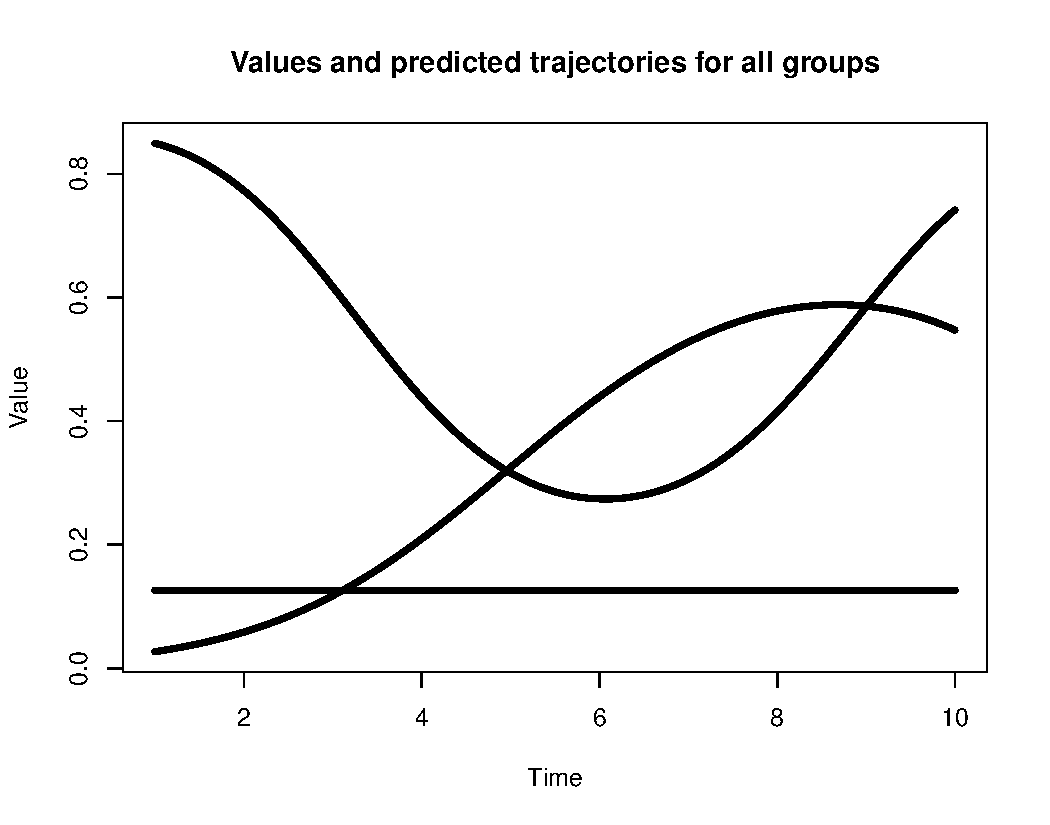
\includegraphics[width=\maxwidth]{figure/unnamed-chunk-11-1} 

\end{knitrout}
We can add longitudinal data to this graph.
If we want this on the plot we have to specify Y and A in the function \verb|plot()|.\\
For more visibility, we have enlarge the 0 and 1 value on the graph and plot the data with a little and random shift, control by the index \verb|dec| in the function plot.\\

By default colors are gray scale, but we can specify colors we want.

\begin{knitrout}
\definecolor{shadecolor}{rgb}{0.969, 0.969, 0.969}\color{fgcolor}\begin{kframe}
\begin{alltt}
\hlcom{# colour's defintion}
\hlstd{trans} \hlkwb{=} \hlstr{"70"}
\hlstd{col1} \hlkwb{=} \hlstr{"#034569"}
\hlstd{col1.1} \hlkwb{=} \hlkwd{paste0}\hlstd{(}\hlstr{"#64AAD0"}\hlstd{, trans)}
\hlstd{col2} \hlkwb{=} \hlstr{"#750062"}
\hlstd{col2.1} \hlkwb{=} \hlkwd{paste0}\hlstd{(}\hlstr{"#D962C7"}\hlstd{, trans)}
\hlstd{col3} \hlkwb{=} \hlstr{"#A68900"}
\hlstd{col3.1} \hlkwb{=} \hlkwd{paste0}\hlstd{(}\hlstr{"#FFE773"}\hlstd{, trans)}
\hlstd{cols1} \hlkwb{=} \hlkwd{c}\hlstd{(col1.1, col2.1, col3.1)}
\hlstd{cols2} \hlkwb{=} \hlkwd{c}\hlstd{(col1, col2, col3)}
\hlstd{vcol} \hlkwb{=} \hlkwd{c}\hlstd{(cols1, cols2)}

\hlkwd{plot}\hlstd{(solLRisk,} \hlkwc{Y} \hlstd{= data[,}\hlnum{2}\hlopt{:}\hlnum{11}\hlstd{],} \hlkwc{A} \hlstd{= data[,}\hlnum{12}\hlopt{:}\hlnum{21}\hlstd{],} \hlkwc{dec} \hlstd{=} \hlnum{5}\hlstd{,} \hlkwc{col} \hlstd{= vcol)}
\end{alltt}
\end{kframe}
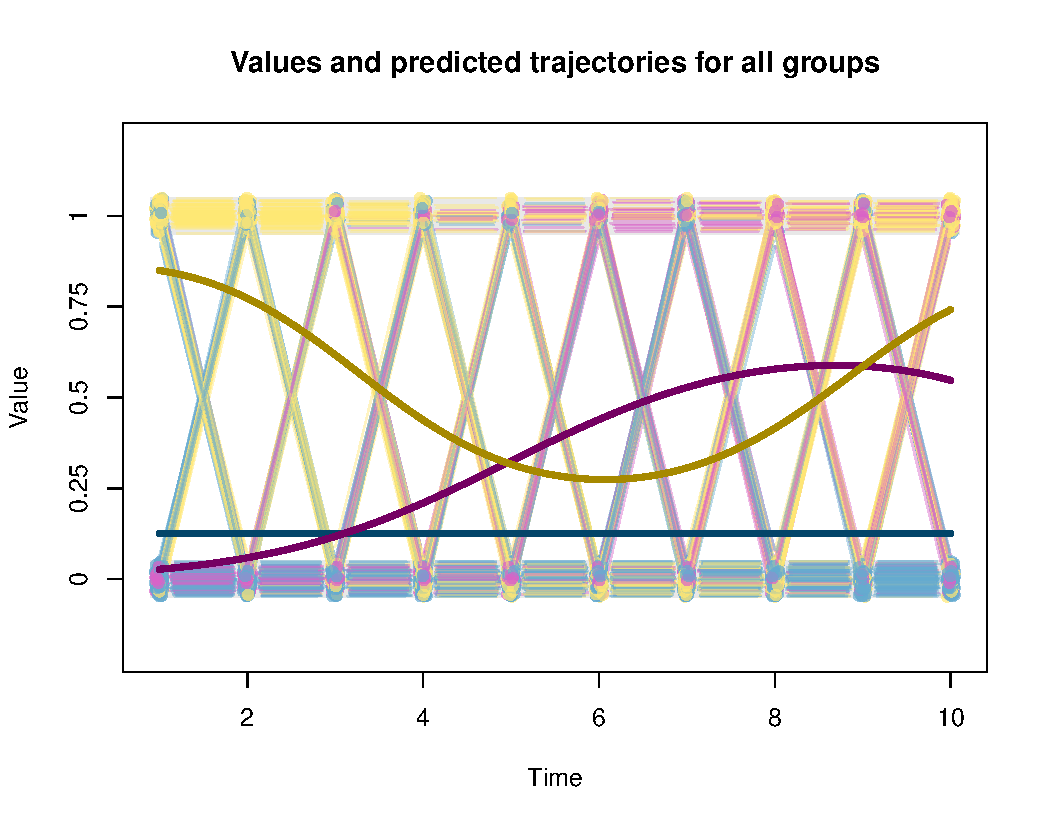
\includegraphics[width=\maxwidth]{figure/unnamed-chunk-12-1} 

\end{knitrout}
We can add the average of the data points on the plot for each time values. For each group and each time the mean of the data are calculated and add to the plot.\\

We use option mean =TRUE.
\begin{knitrout}
\definecolor{shadecolor}{rgb}{0.969, 0.969, 0.969}\color{fgcolor}\begin{kframe}
\begin{alltt}
\hlcom{# colour's defintion}
\hlstd{trans} \hlkwb{=} \hlstr{"70"}
\hlstd{col1} \hlkwb{=} \hlstr{"#034569"}
\hlstd{col1.1} \hlkwb{=} \hlkwd{paste0}\hlstd{(}\hlstr{"#64AAD0"}\hlstd{, trans)}
\hlstd{col2} \hlkwb{=} \hlstr{"#750062"}
\hlstd{col2.1} \hlkwb{=} \hlkwd{paste0}\hlstd{(}\hlstr{"#D962C7"}\hlstd{, trans)}
\hlstd{col3} \hlkwb{=} \hlstr{"#A68900"}
\hlstd{col3.1} \hlkwb{=} \hlkwd{paste0}\hlstd{(}\hlstr{"#FFE773"}\hlstd{, trans)}
\hlstd{cols1} \hlkwb{=} \hlkwd{c}\hlstd{(col1.1, col2.1, col3.1)}
\hlstd{cols2} \hlkwb{=} \hlkwd{c}\hlstd{(col1, col2, col3)}
\hlstd{vcol} \hlkwb{=} \hlkwd{c}\hlstd{(cols1, cols2)}

\hlkwd{plot}\hlstd{(solLRisk,} \hlkwc{Y} \hlstd{= data[,}\hlnum{2}\hlopt{:}\hlnum{11}\hlstd{],} \hlkwc{A} \hlstd{= data[,}\hlnum{12}\hlopt{:}\hlnum{21}\hlstd{],} \hlkwc{dec} \hlstd{=} \hlnum{5}\hlstd{,}
     \hlkwc{col} \hlstd{= vcol,} \hlkwc{mean} \hlstd{=} \hlnum{TRUE}\hlstd{,} \hlkwc{alpha} \hlstd{=} \hlnum{0.3}\hlstd{)}
\end{alltt}
\end{kframe}
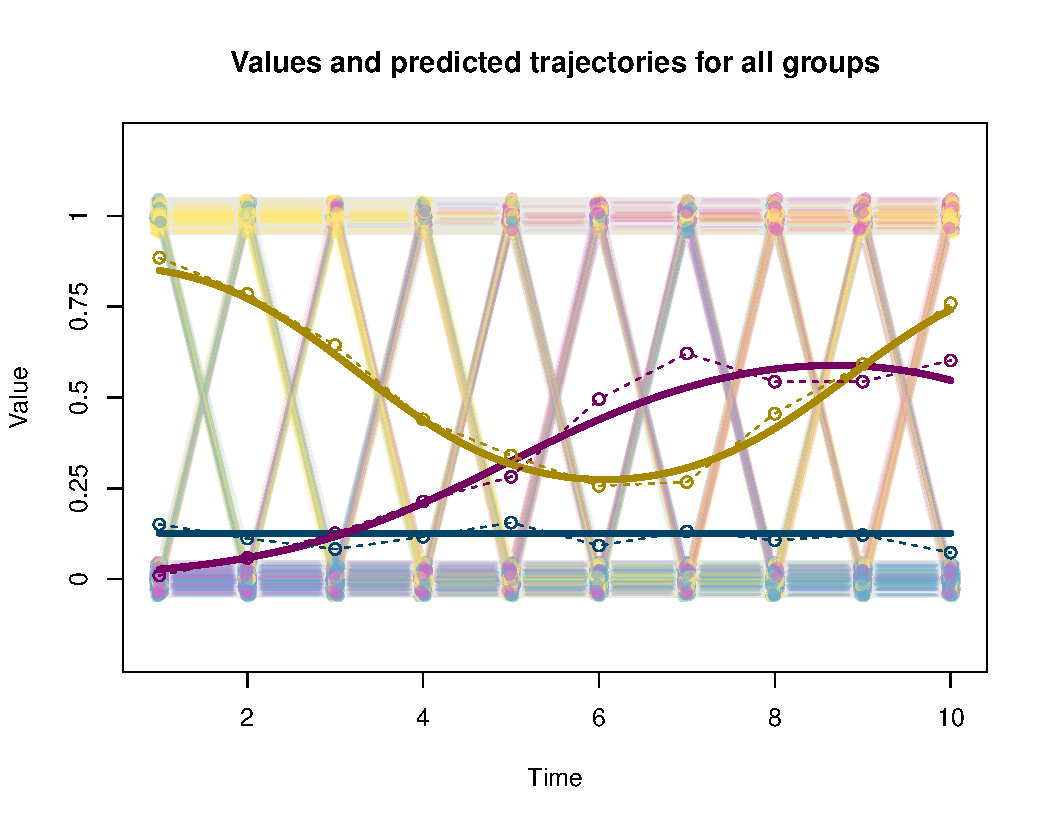
\includegraphics[width=\maxwidth]{figure/unnamed-chunk-13-1} 

\end{knitrout}

Time covariate can influenced directly the shape trajectory. In the data, we have time covariate that is composed by 0 or 1 value. We consider their effects by use the option \verb|TCOV| in the command trajeR. We can use any of three method above.

\begin{knitrout}
\definecolor{shadecolor}{rgb}{0.969, 0.969, 0.969}\color{fgcolor}\begin{kframe}
\begin{alltt}
\hlstd{solLTCOV} \hlkwb{=} \hlkwd{trajeR}\hlstd{(}\hlkwc{Y} \hlstd{= data[,}\hlnum{2}\hlopt{:}\hlnum{11}\hlstd{],} \hlkwc{A} \hlstd{=data[,}\hlnum{12}\hlopt{:}\hlnum{21}\hlstd{],} \hlkwc{TCOV} \hlstd{= data[,}\hlnum{24}\hlopt{:}\hlnum{33}\hlstd{],}
                  \hlkwc{ng} \hlstd{=} \hlnum{3}\hlstd{,} \hlkwc{degre} \hlstd{=} \hlkwd{c}\hlstd{(}\hlnum{0}\hlstd{,}\hlnum{3}\hlstd{,}\hlnum{4}\hlstd{),}
                  \hlkwc{Model} \hlstd{=} \hlstr{"LOGIT"}\hlstd{,} \hlkwc{Method} \hlstd{=} \hlstr{"L"}\hlstd{,} \hlkwc{hessian} \hlstd{=} \hlnum{TRUE}\hlstd{,}
                  \hlkwc{itermax} \hlstd{=} \hlnum{300}\hlstd{,} \hlkwc{paraminit} \hlstd{= paraminit)}
\hlstd{solEMTCOV} \hlkwb{=} \hlkwd{trajeR}\hlstd{(}\hlkwc{Y} \hlstd{= data[,}\hlnum{2}\hlopt{:}\hlnum{11}\hlstd{],} \hlkwc{A} \hlstd{= data[,}\hlnum{12}\hlopt{:}\hlnum{21}\hlstd{],} \hlkwc{TCOV} \hlstd{= data[,}\hlnum{24}\hlopt{:}\hlnum{33}\hlstd{],}
                   \hlkwc{ng} \hlstd{=} \hlnum{3}\hlstd{,} \hlkwc{degre} \hlstd{=} \hlkwd{c}\hlstd{(}\hlnum{0}\hlstd{,}\hlnum{3}\hlstd{,}\hlnum{4}\hlstd{),}
                   \hlkwc{Model} \hlstd{=} \hlstr{"LOGIT"}\hlstd{,} \hlkwc{Method} \hlstd{=} \hlstr{"EM"}\hlstd{,} \hlkwc{hessian} \hlstd{=} \hlnum{FALSE}\hlstd{,}
                   \hlkwc{itermax} \hlstd{=} \hlnum{300}\hlstd{,} \hlkwc{paraminit} \hlstd{= paraminit)}
\hlstd{solEMIWRLSTCOV} \hlkwb{=} \hlkwd{trajeR}\hlstd{(}\hlkwc{Y} \hlstd{= data[,}\hlnum{2}\hlopt{:}\hlnum{11}\hlstd{],} \hlkwc{A} \hlstd{= data[,}\hlnum{12}\hlopt{:}\hlnum{21}\hlstd{],} \hlkwc{TCOV} \hlstd{= data[,}\hlnum{24}\hlopt{:}\hlnum{33}\hlstd{],}
                        \hlkwc{ng} \hlstd{=} \hlnum{3}\hlstd{,} \hlkwc{degre} \hlstd{=} \hlkwd{c}\hlstd{(}\hlnum{0}\hlstd{,}\hlnum{3}\hlstd{,}\hlnum{4}\hlstd{),}
                        \hlkwc{Model} \hlstd{=} \hlstr{"LOGIT"}\hlstd{,} \hlkwc{Method} \hlstd{=} \hlstr{"EMIWRLS"}\hlstd{,} \hlkwc{hessian} \hlstd{=} \hlnum{FALSE}\hlstd{,}
                        \hlkwc{itermax} \hlstd{=} \hlnum{300}\hlstd{,} \hlkwc{paraminit} \hlstd{= paraminit)}
\end{alltt}
\end{kframe}
\end{knitrout}
\begin{knitrout}
\definecolor{shadecolor}{rgb}{0.969, 0.969, 0.969}\color{fgcolor}\begin{kframe}
\begin{alltt}
\hlstd{solLTCOV}
\end{alltt}
\begin{verbatim}
## Call TrajeR with 3 groups and a 0,3,4 degrees of polynomial shape of trajectory.
## Model : Logit
## Method : Likelihood 
##  
##   group   Parameter   Estimate   Std. Error   T for H0:   Prob>|T|  
##                                                param.=0             
## --------------------------------------------------------------------
##       1   Intercept   -2.01704       0.1416   -14.24421          0  
##               TCOV1    0.14154      0.17273     0.81945    0.41257  
##                                                                     
##       2   Intercept   -1.84758      0.04094   -45.13106          0  
##              Linear   -0.42841          NaN         NaN        NaN  
##           Quadratic    0.18461          NaN         NaN        NaN  
##               Cubic    -0.0122          NaN         NaN        NaN  
##               TCOV1    0.12146      0.19278     0.63002    0.52871  
##                                                                     
##       3   Intercept    1.72074          NaN         NaN        NaN  
##              Linear    0.66231      0.08125     8.15111          0  
##           Quadratic   -0.56112      0.02615   -21.45863          0  
##               Cubic    0.08274      0.00202    40.88649          0  
##           Quadratic   -0.00339          NaN         NaN        NaN  
##               TCOV1    0.01848       0.1141     0.16196    0.87134  
## --------------------------------------------------------------------
##       1         pi1    0.41873      0.10831     2.44733    0.01443  
##       2         pi2    0.21778      0.11333    -3.42939    0.00061  
##       3         pi3    0.36348      0.06309     1.95879    0.05019  
## --------------------------------------------------------------------
## Likelihood : -2851.937
\end{verbatim}
\begin{alltt}
\hlstd{solEMTCOV}
\end{alltt}
\begin{verbatim}
## Call TrajeR with 3 groups and a 0,3,4 degrees of polynomial shape of trajectory.
## Model : Logit
## Method : Expectation-maximization 
##  
##   group   Parameter   Estimate   Std. Error   T for H0:   Prob>|T|  
##                                                param.=0             
## --------------------------------------------------------------------
##       1   Intercept   -2.07354           NA          NA         NA  
##               TCOV1    0.18405           NA          NA         NA  
##                                                                     
##       2   Intercept   -1.49687           NA          NA         NA  
##              Linear   -0.57226           NA          NA         NA  
##           Quadratic    0.20213           NA          NA         NA  
##               Cubic   -0.01287           NA          NA         NA  
##               TCOV1    0.09458           NA          NA         NA  
##                                                                     
##       3   Intercept     1.7166           NA          NA         NA  
##              Linear    0.71904           NA          NA         NA  
##           Quadratic   -0.58235           NA          NA         NA  
##               Cubic    0.08523           NA          NA         NA  
##           Quadratic   -0.00348           NA          NA         NA  
##               TCOV1    0.01717           NA          NA         NA  
## --------------------------------------------------------------------
##       1         pi1     0.4102           NA          NA         NA  
##       2         pi2    0.23247           NA          NA         NA  
##       3         pi3    0.35732           NA          NA         NA  
## --------------------------------------------------------------------
## Likelihood : -2855.357
\end{verbatim}
\begin{alltt}
\hlstd{solEMIWRLSTCOV}
\end{alltt}
\begin{verbatim}
## Call TrajeR with 3 groups and a 0,3,4 degrees of polynomial shape of trajectory.
## Model : Logit
## Method : Expectation-maximization with IWRLS
##  
##   group   Parameter   Estimate   Std. Error   T for H0:   Prob>|T|  
##                                                param.=0             
## --------------------------------------------------------------------
##       1   Intercept   -2.01725           NA          NA         NA  
##               TCOV1    0.14188           NA          NA         NA  
##                                                                     
##       2   Intercept   -1.84956           NA          NA         NA  
##              Linear   -0.42662           NA          NA         NA  
##           Quadratic    0.18422           NA          NA         NA  
##               Cubic   -0.01217           NA          NA         NA  
##               TCOV1    0.11965           NA          NA         NA  
##                                                                     
##       3   Intercept    1.72138           NA          NA         NA  
##              Linear    0.66141           NA          NA         NA  
##           Quadratic    -0.5608           NA          NA         NA  
##               Cubic     0.0827           NA          NA         NA  
##           Quadratic   -0.00339           NA          NA         NA  
##               TCOV1    0.01868           NA          NA         NA  
## --------------------------------------------------------------------
##       1         pi1     0.4187           NA          NA         NA  
##       2         pi2    0.21781           NA          NA         NA  
##       3         pi3     0.3635           NA          NA         NA  
## --------------------------------------------------------------------
## Likelihood : -2856.402
\end{verbatim}
\end{kframe}
\end{knitrout}
\begin{knitrout}
\definecolor{shadecolor}{rgb}{0.969, 0.969, 0.969}\color{fgcolor}\begin{kframe}
\begin{alltt}
\hlkwd{plot}\hlstd{(solLTCOV,} \hlkwc{col} \hlstd{= vcol)}
\end{alltt}
\end{kframe}
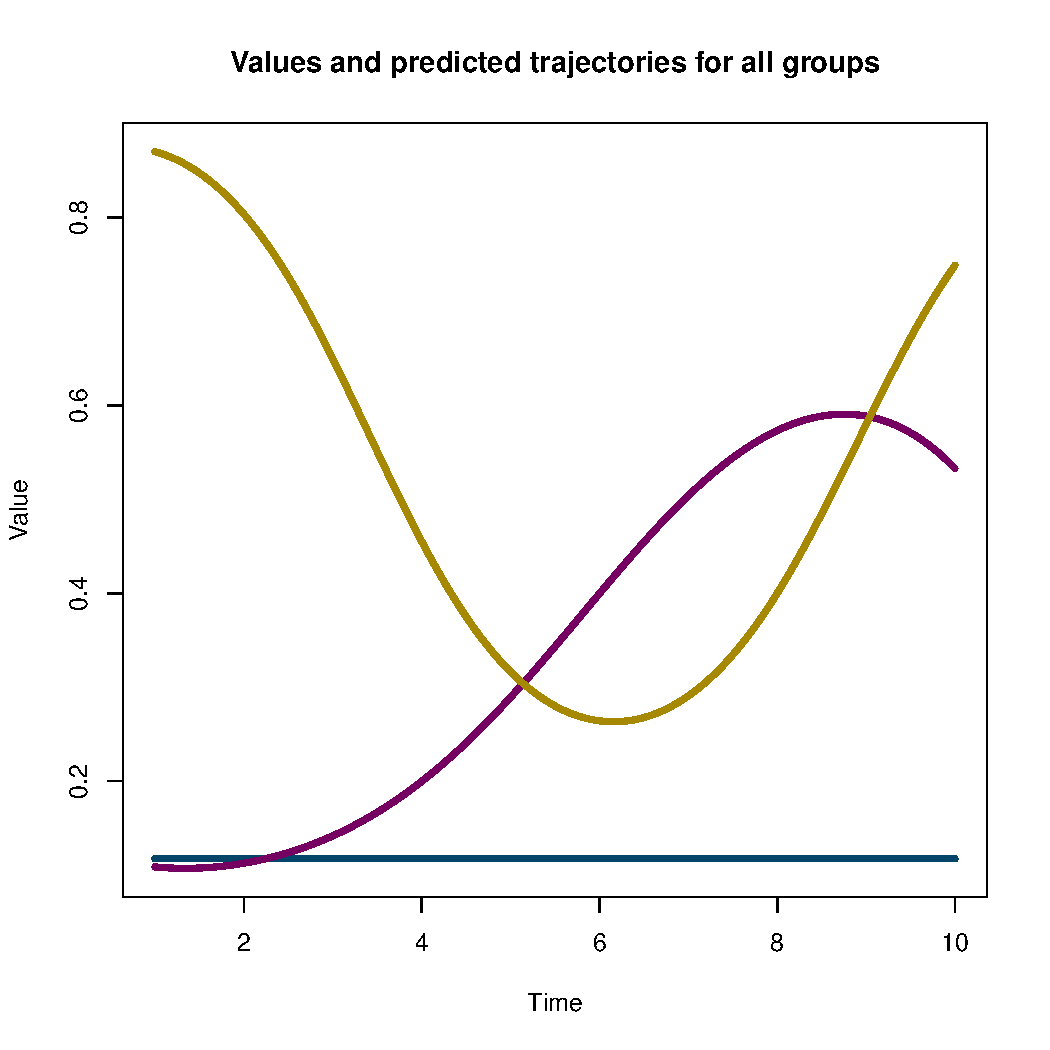
\includegraphics[width=\maxwidth]{figure/unnamed-chunk-16-1} 

\end{knitrout}

If we want show the impact of a particular value of the time covariate in the trajectory, we can add this to the plot by \verb|plotcov| option.\\
The fill line is the trajectory with the time covariate matrix and th dashed one show the impact on this trajectory of a particular value.
\begin{knitrout}
\definecolor{shadecolor}{rgb}{0.969, 0.969, 0.969}\color{fgcolor}\begin{kframe}
\begin{alltt}
\hlkwd{plot}\hlstd{(solLTCOV,} \hlkwc{col} \hlstd{= vcol,} \hlkwc{plotcov} \hlstd{=} \hlkwd{c}\hlstd{(}\hlnum{0}\hlstd{,}\hlnum{0}\hlstd{,}\hlnum{0}\hlstd{,}\hlnum{0}\hlstd{,}\hlnum{0}\hlstd{,}\hlnum{1}\hlstd{,}\hlnum{1}\hlstd{,}\hlnum{1}\hlstd{,}\hlnum{1}\hlstd{,}\hlnum{1}\hlstd{))}
\end{alltt}
\end{kframe}
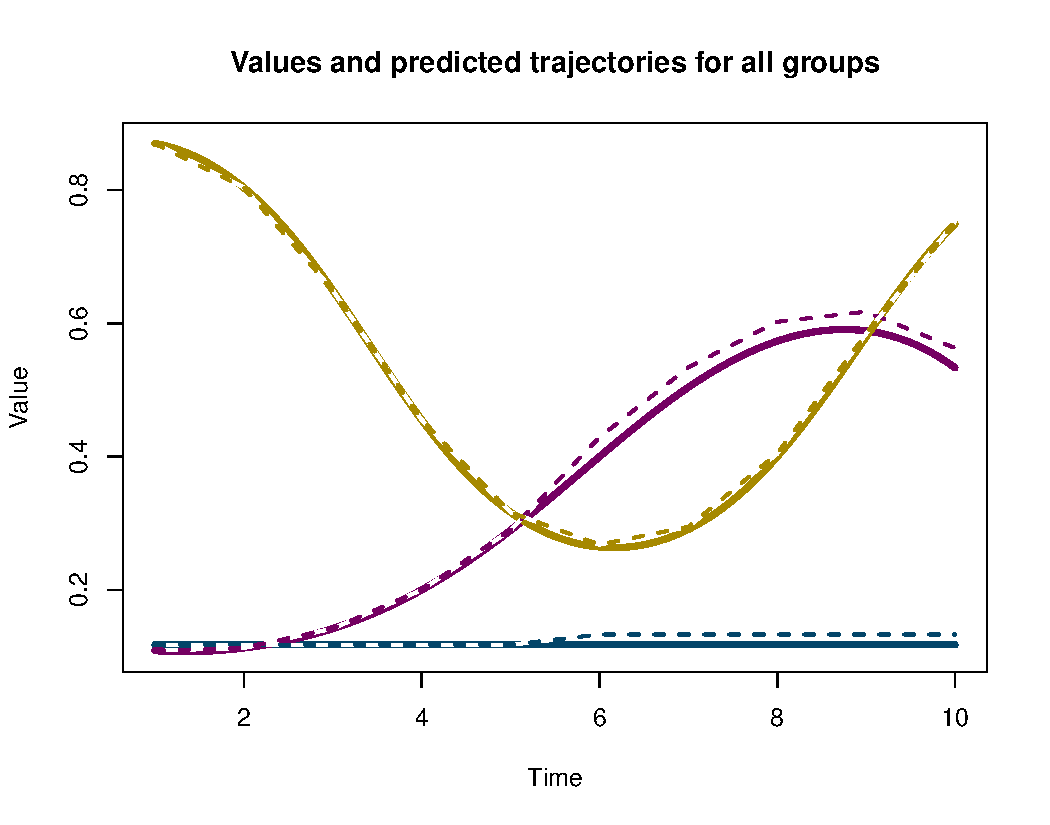
\includegraphics[width=\maxwidth]{figure/unnamed-chunk-17-1} 

\end{knitrout}


\section{Censored Normal distribution}

To illustrate this party we use aritifial data contained in this package \verb|CNORM_data01|.

\section{Censored Normal model}
We suppose that the variable $Y_{it}$ is a censored variable, i.e. its values are between two numbers $y_{min}$ and $y_{max}$.\\
We consider a variable $Y^*_{it}$ that is normally distributed and such
\begin{equation}
y^*_{it} = f(a_{it}; \beta_k, \delta_k)+\epsilon_{it} =\beta_k A_{it}+\delta_k W_t+\epsilon_{it}
\end{equation}
where $\epsilon_{it}\sim \mathcal{N}\left(0;\ \sigma\right)$,  $A_{it}=(1,a_{it},a_{it}^2,\cdots,a_{it}^{n_\beta-1})^t $, $W_t=(w_{i1},\cdots,w_{in_\delta})^t $, $\beta_k =(\beta_{k1},\cdots, \beta_{kn_\beta})$ and $\delta_k=(\delta_{k1},\cdots,\delta_{kn_\delta}) $\\
Furthermore, we can link $y^*_{it}$ to the observed and censored data $y_{it}$.
\begin{align}
& y_{it}= y_{min} \text{ if } y^*_{it}< y_{min}\\
& y_{it}= y^*_{it} \text{ if } y_{min}\leq y^*_{it}\leq y_{max}\\
&y_{it}= y_{max} \text{ if } y^*_{it}> y_{max}\\
\end{align}

By asking $\mu_{ikt}=\beta_k A_{it}+\delta_k W_t$,  we can write
\begin{align}
P(Y_{it}=y_{it}|W_i=w_i,C_i=k)=\left\lbrace
\begin{array}{l}
\Phi\left(\dfrac{y_{min}-\mu_{ikt}}{\sigma_k}\right) \text{ if } y^*_{it}< y_{min}\\
\dfrac{1}{\sigma_k}\phi\left(\dfrac{y_{it}-\mu_{ikt}}{\sigma_k}\right)\text{ if } y_{min}\leq y^*_{it}\leq y_{max}\\
1-\Phi\left(\dfrac{y_{max}-\mu_{ikt}}{\sigma_k}\right) \text{ if } y^*_{it}> y_{max}
\end{array}\right.
\end{align}

\subsection{Parameters}

\textbf{Example}\\
We use artificial data contained in the library. This are 500 longitudinal data generate by the parameters above :
\begin{itemize}
	\item 3 groups ;
	\item probability is $\pi_1=0.32$, $\pi_2=0.54$ and $\pi_3=0.14$ ;
	\item period is 10 ;
	\item we use 3 polynomial shape
	\begin{enumerate}
		\item degre 3 and $\beta_1=(2.797,8.809,-3.201,0.463,-0.021)$ ;
		\item degre 4 and $\beta_2=7$ ;
		\item degre 0 and $\beta_{3}=(19.545,-0.297,-0.407,0.026)$.
	\end{enumerate}
	\item $\sigma$ is the same for the 3 groups, $\sigma= 4$.
\end{itemize}

The data contained the time variable dependent $Y_i$ in \verb|data[,2:11]|, the time variable in \verb|data[,12:21]|, the time covariate in \verb|data[,22:41]| and a covariate that influence the belonging probabilty in \verb|data[,42:43]|.
\begin{itemize}
	\item \verb|data[,2:11]| is a matrix withe real.
	\item \verb|data[,12:21]| is a matrix with time 1 to 10.
	\item \verb|data[,22:31]| is a time covriate that influence the shape fo trajectory. It is a matrix with 0 and 1 value, like the presence or not of a characteristic on the individual.
	\item \verb|data[,32:41]| is a time covriate that influence the shape fo trajectory. It is a matrix with real.
	\item \verb|data[,42:43]| is a matrix with real.
\end{itemize}



\begin{knitrout}
\definecolor{shadecolor}{rgb}{0.969, 0.969, 0.969}\color{fgcolor}
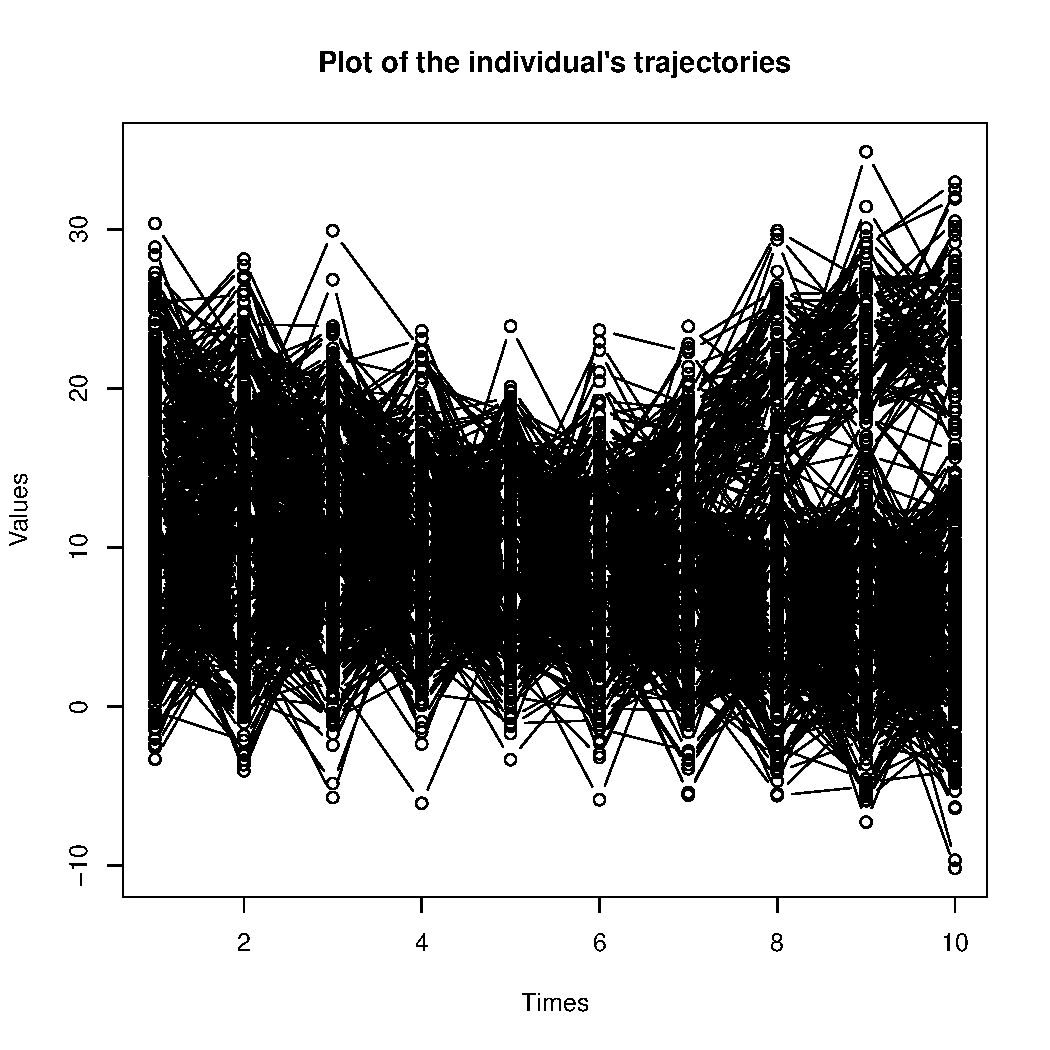
\includegraphics[width=\maxwidth]{figure/unnamed-chunk-19-1} 

\end{knitrout}
We use the each method to fit the model. For all method, we specifies the number of group of our model, ng=3, the degree of the polynomial of the shape of the trajectory. Here we choice a line parallel to abscissa axis, a cubic polynomial and a quadric polynomial. So degree is a vector $(0,3,4)$.\\
We sepcifie \verb|hessian=TRUE| to ask the calculus of the hessian matrix.\\
\verb|Itermax | is set to 300 to assure a good approximation of the parameters.\\

For the Likelihood method we call trajeR with option Method ="L". We speicfy if we want the same sigma in each group with the parameters \verb|\ssigma|. If it is \verb|TRUE| the the algorithm surch the same sigma in all group.

\begin{knitrout}
\definecolor{shadecolor}{rgb}{0.969, 0.969, 0.969}\color{fgcolor}\begin{kframe}
\begin{alltt}
\hlcom{# Likelihood different sigma}
\hlstd{solL} \hlkwb{=} \hlkwd{trajeR}\hlstd{(}\hlkwc{Y} \hlstd{= data[,}\hlnum{2}\hlopt{:}\hlnum{11}\hlstd{],} \hlkwc{A} \hlstd{= data[,}\hlnum{12}\hlopt{:}\hlnum{21}\hlstd{],}
              \hlkwc{ng} \hlstd{=} \hlnum{3}\hlstd{,} \hlkwc{degre} \hlstd{=} \hlkwd{c}\hlstd{(}\hlnum{0}\hlstd{,}\hlnum{3}\hlstd{,}\hlnum{4}\hlstd{),}
              \hlkwc{Model} \hlstd{=} \hlstr{"CNORM"}\hlstd{,} \hlkwc{Method} \hlstd{=} \hlstr{"EM"}\hlstd{,}  \hlkwc{hessian} \hlstd{=} \hlnum{FALSE}\hlstd{,} \hlkwc{ssigma} \hlstd{=} \hlnum{FALSE}\hlstd{)}
\end{alltt}
\end{kframe}
\end{knitrout}
\begin{knitrout}
\definecolor{shadecolor}{rgb}{0.969, 0.969, 0.969}\color{fgcolor}\begin{kframe}
\begin{alltt}
\hlstd{solL}
\end{alltt}
\begin{verbatim}
## Call TrajeR with 3 groups and a 0,3,4 degrees of polynomial shape of trajectory.
## Model : Censored Normal
## Method : Likelihood 
##  
##   group   Parameter   Estimate   Std. Error   T for H0:   Prob>|T|  
##                                                param.=0             
## --------------------------------------------------------------------
##       1   Intercept    7.04989      0.08425    83.67725          0  
##                                                                     
##       2   Intercept    19.3042      0.08322   231.96629          0  
##              Linear   -0.09337      0.10609    -0.88009    0.37885  
##           Quadratic   -0.45605      0.03793   -12.02404          0  
##               Cubic    0.02918      0.00287    10.16725          0  
##                                                                     
##       3   Intercept    1.66272      0.01264   131.55795          0  
##              Linear   10.12613      0.02797   362.03353          0  
##           Quadratic   -3.71001      0.04415   -84.02376          0  
##               Cubic    0.53801      0.01303    41.28388          0  
##             Quartic    -0.0246      0.00087   -28.35329          0  
## --------------------------------------------------------------------
##       1      sigma1     3.9581      0.01522   260.00927          0  
##       2      sigma2    4.11023      0.01714    239.8676          0  
##       3      sigma3    4.00186      0.02338   171.14613          0  
## --------------------------------------------------------------------
##       1         pi1    0.45891       0.0616    22.42831          0  
##       2         pi2    0.34895      0.06515    17.00024          0  
##       3         pi3    0.19214      0.07596     6.72576          0  
## --------------------------------------------------------------------
## Likelihood : -14564.35
\end{verbatim}
\end{kframe}
\end{knitrout}
If we want force use unique sigma for each groups we write \verb|ssigma = TRUE|.
\begin{knitrout}
\definecolor{shadecolor}{rgb}{0.969, 0.969, 0.969}\color{fgcolor}\begin{kframe}
\begin{alltt}
\hlcom{# Likelihood same sigma}
\hlstd{solLs} \hlkwb{=} \hlkwd{trajeR}\hlstd{(}\hlkwc{Y} \hlstd{= data[,}\hlnum{2}\hlopt{:}\hlnum{11}\hlstd{],} \hlkwc{A} \hlstd{= data[,}\hlnum{12}\hlopt{:}\hlnum{21}\hlstd{],}
               \hlkwc{ng} \hlstd{=} \hlnum{3}\hlstd{,} \hlkwc{degre} \hlstd{=} \hlkwd{c}\hlstd{(}\hlnum{0}\hlstd{,}\hlnum{3}\hlstd{,}\hlnum{4}\hlstd{),}
               \hlkwc{Model} \hlstd{=} \hlstr{"CNORM"}\hlstd{,} \hlkwc{Method} \hlstd{=} \hlstr{"EM"}\hlstd{,} \hlkwc{ssigma} \hlstd{=} \hlnum{TRUE}\hlstd{,} \hlkwc{hessian} \hlstd{=} \hlnum{FALSE}\hlstd{)}
\end{alltt}
\end{kframe}
\end{knitrout}
\begin{knitrout}
\definecolor{shadecolor}{rgb}{0.969, 0.969, 0.969}\color{fgcolor}\begin{kframe}
\begin{alltt}
\hlstd{solLs}
\end{alltt}
\begin{verbatim}
## Call TrajeR with 3 groups and a 0,3,4 degrees of polynomial shape of trajectory.
## Model : Censored Normal
## Method : Likelihood 
##  
##   group   Parameter   Estimate   Std. Error   T for H0:   Prob>|T|  
##                                                param.=0             
## --------------------------------------------------------------------
##       1   Intercept    7.05315       0.0851    82.88488          0  
##                                                                     
##       2   Intercept   19.31443      0.07947   243.05329          0  
##              Linear   -0.08916      0.10115    -0.88145    0.37812  
##           Quadratic   -0.45758      0.03641   -12.56655          0  
##               Cubic    0.02928      0.00277     10.5622          0  
##                                                                     
##       3   Intercept    1.67003      0.01209   138.08107          0  
##              Linear   10.11777      0.02697   375.19146          0  
##           Quadratic   -3.70707      0.04374   -84.75415          0  
##               Cubic    0.53762      0.01283    41.89705          0  
##             Quartic   -0.02459      0.00085    -28.7909          0  
## --------------------------------------------------------------------
##       1      sigma1    4.02025          NaN         NaN        NaN  
##       2      sigma2    4.02025      0.01864   215.70733          0  
##       3      sigma3    4.02025          NaN         NaN        NaN  
## --------------------------------------------------------------------
##       1         pi1    0.45979      0.06143    22.52374          0  
##       2         pi2    0.34813      0.06501    17.00387          0  
##       3         pi3    0.19208        0.076     6.72199          0  
## --------------------------------------------------------------------
## Likelihood : -14565.75
\end{verbatim}
\end{kframe}
\end{knitrout}
For use EM method we write the same syntax but change the variable \verb|Method| to \verb|EM|.
\begin{knitrout}
\definecolor{shadecolor}{rgb}{0.969, 0.969, 0.969}\color{fgcolor}\begin{kframe}
\begin{alltt}
\hlcom{# EM}
\hlstd{solEM} \hlkwb{=} \hlkwd{trajeR}\hlstd{(}\hlkwc{Y} \hlstd{= data[,}\hlnum{2}\hlopt{:}\hlnum{11}\hlstd{],} \hlkwc{A} \hlstd{= data[,}\hlnum{12}\hlopt{:}\hlnum{21}\hlstd{],}
               \hlkwc{ng} \hlstd{=} \hlnum{3}\hlstd{,} \hlkwc{degre} \hlstd{=} \hlkwd{c}\hlstd{(}\hlnum{0}\hlstd{,}\hlnum{3}\hlstd{,}\hlnum{4}\hlstd{),}
               \hlkwc{Model} \hlstd{=} \hlstr{"CNORM"}\hlstd{,} \hlkwc{Method} \hlstd{=} \hlstr{"EM"}\hlstd{,} \hlkwc{ssigma} \hlstd{=} \hlnum{FALSE}\hlstd{,} \hlkwc{hessian} \hlstd{=} \hlnum{FALSE}\hlstd{)}
\hlstd{solEMs} \hlkwb{=} \hlkwd{trajeR}\hlstd{(}\hlkwc{Y} \hlstd{= data[,}\hlnum{2}\hlopt{:}\hlnum{11}\hlstd{],} \hlkwc{A} \hlstd{= data[,}\hlnum{12}\hlopt{:}\hlnum{21}\hlstd{],}
                \hlkwc{ng} \hlstd{=} \hlnum{3}\hlstd{,} \hlkwc{degre} \hlstd{=} \hlkwd{c}\hlstd{(}\hlnum{0}\hlstd{,}\hlnum{3}\hlstd{,}\hlnum{4}\hlstd{),}
                \hlkwc{Model} \hlstd{=} \hlstr{"CNORM"}\hlstd{,} \hlkwc{Method} \hlstd{=} \hlstr{"EM"}\hlstd{,} \hlkwc{ssigma} \hlstd{=} \hlnum{TRUE}\hlstd{,} \hlkwc{hessian} \hlstd{=} \hlnum{FALSE}\hlstd{)}
\end{alltt}
\end{kframe}
\end{knitrout}


\begin{table}[H]
\centering
\begin{tabular}{rrrr}
\toprule
\multicolumn{2}{c}{Different sigma} & \multicolumn{2}{c}{Same sigma} \\
\cmidrule(l{3pt}r{3pt}){1-2} \cmidrule(l{3pt}r{3pt}){3-4}
SolL & SolEM & SolLs & SolEMs\\
\midrule
\addlinespace[0.3em]
\multicolumn{4}{l}{\textbf{Beta 1}}\\
\hspace{1em}7.04989 & 7.04940 & 7.05315 & 7.05316\\
\addlinespace[0.3em]
\multicolumn{4}{l}{\textbf{Beta 2}}\\
\hspace{1em}19.30420 & 19.30454 & 19.31443 & 19.31467\\
\hspace{1em}-0.09337 & -0.09315 & -0.08916 & -0.08935\\
\hspace{1em}-0.45605 & -0.45614 & -0.45758 & -0.45753\\
\hspace{1em}0.02918 & 0.02919 & 0.02928 & 0.02927\\
\addlinespace[0.3em]
\multicolumn{4}{l}{\textbf{Beta 3}}\\
\hspace{1em}1.66272 & 1.66950 & 1.67003 & 1.66950\\
\hspace{1em}10.12613 & 10.11827 & 10.11777 & 10.11834\\
\hspace{1em}-3.71001 & -3.70726 & -3.70707 & -3.70726\\
\hspace{1em}0.53801 & 0.53764 & 0.53762 & 0.53764\\
\hspace{1em}-0.02460 & -0.02459 & -0.02459 & -0.02459\\
\addlinespace[0.3em]
\multicolumn{4}{l}{\textbf{Sigma}}\\
\hspace{1em}3.95810 & 3.95795 & 4.02025 & 4.02028\\
\hspace{1em}4.11023 & 4.11085 & 4.02025 & 4.02028\\
\hspace{1em}4.00186 & 4.00173 & 4.02025 & 4.02028\\
\addlinespace[0.3em]
\multicolumn{4}{l}{\textbf{Pi}}\\
\hspace{1em}0.45891 & 0.45891 & 0.45979 & 0.45978\\
\hspace{1em}0.34895 & 0.34901 & 0.34813 & 0.34814\\
\hspace{1em}0.19214 & 0.19208 & 0.19208 & 0.19207\\
\bottomrule
\end{tabular}
\end{table}


\label{probCens}
\subsection{Plot}
We plot only the trajectory on a graph. We have just to use the native plot function. It use the class of the object to draw the polynomial shape. The values in abscissa are the first row of the time variable.

\begin{knitrout}
\definecolor{shadecolor}{rgb}{0.969, 0.969, 0.969}\color{fgcolor}\begin{kframe}
\begin{alltt}
\hlkwd{plot}\hlstd{(solL)}
\end{alltt}
\end{kframe}
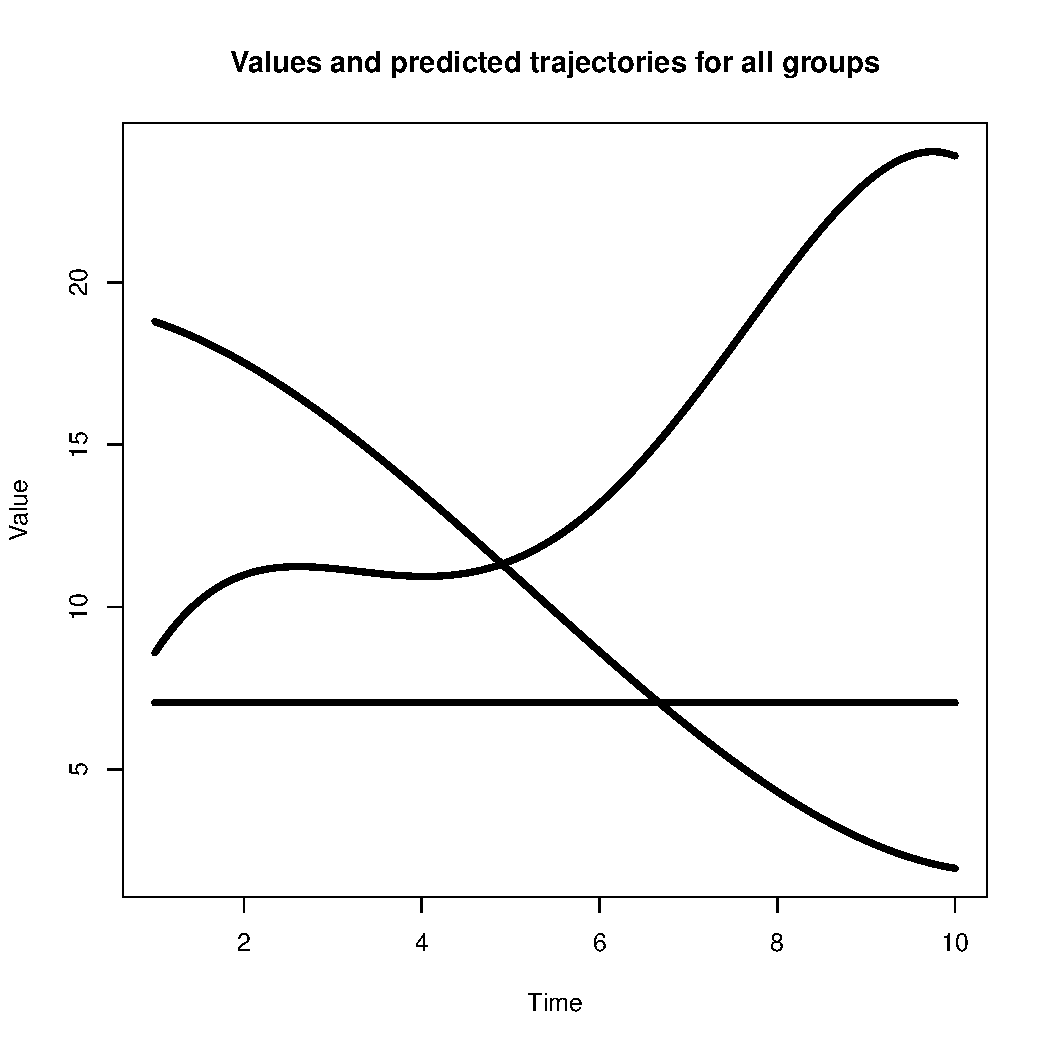
\includegraphics[width=\maxwidth]{figure/unnamed-chunk-27-1} 

\end{knitrout}
We can add longitudinal data to this graph. If we want this on the plot we have to specify \verb|Y| and \verb|A| in the function \verb|plot()|. For more visibility, we have enlarge the 0 and 1 value on the graph and plot the data with a little and random shift, control by the index dec in the function plot.\\
By default colors are gray scale, but we can specify colors we want.

\begin{knitrout}
\definecolor{shadecolor}{rgb}{0.969, 0.969, 0.969}\color{fgcolor}\begin{kframe}
\begin{alltt}
\hlcom{# colour's defintion}
\hlstd{trans} \hlkwb{=} \hlstr{"70"}
\hlstd{col1} \hlkwb{=} \hlstr{"#034569"}
\hlstd{col1.1} \hlkwb{=} \hlkwd{paste0}\hlstd{(}\hlstr{"#64AAD0"}\hlstd{, trans)}
\hlstd{col2} \hlkwb{=} \hlstr{"#750062"}
\hlstd{col2.1} \hlkwb{=} \hlkwd{paste0}\hlstd{(}\hlstr{"#D962C7"}\hlstd{, trans)}
\hlstd{col3} \hlkwb{=} \hlstr{"#A68900"}
\hlstd{col3.1} \hlkwb{=} \hlkwd{paste0}\hlstd{(}\hlstr{"#FFE773"}\hlstd{, trans)}
\hlstd{cols1} \hlkwb{=} \hlkwd{c}\hlstd{(col1.1, col2.1, col3.1)}
\hlstd{cols2} \hlkwb{=} \hlkwd{c}\hlstd{(col1, col2, col3)}
\hlstd{vcol} \hlkwb{=} \hlkwd{c}\hlstd{(cols1, cols2)}

\hlkwd{plot}\hlstd{(solEM,} \hlkwc{Y} \hlstd{= data[,}\hlnum{2}\hlopt{:}\hlnum{11}\hlstd{],} \hlkwc{A} \hlstd{= data[,}\hlnum{12}\hlopt{:}\hlnum{21}\hlstd{],} \hlkwc{dec} \hlstd{=} \hlnum{5}\hlstd{,} \hlkwc{col} \hlstd{= vcol)}
\end{alltt}
\end{kframe}
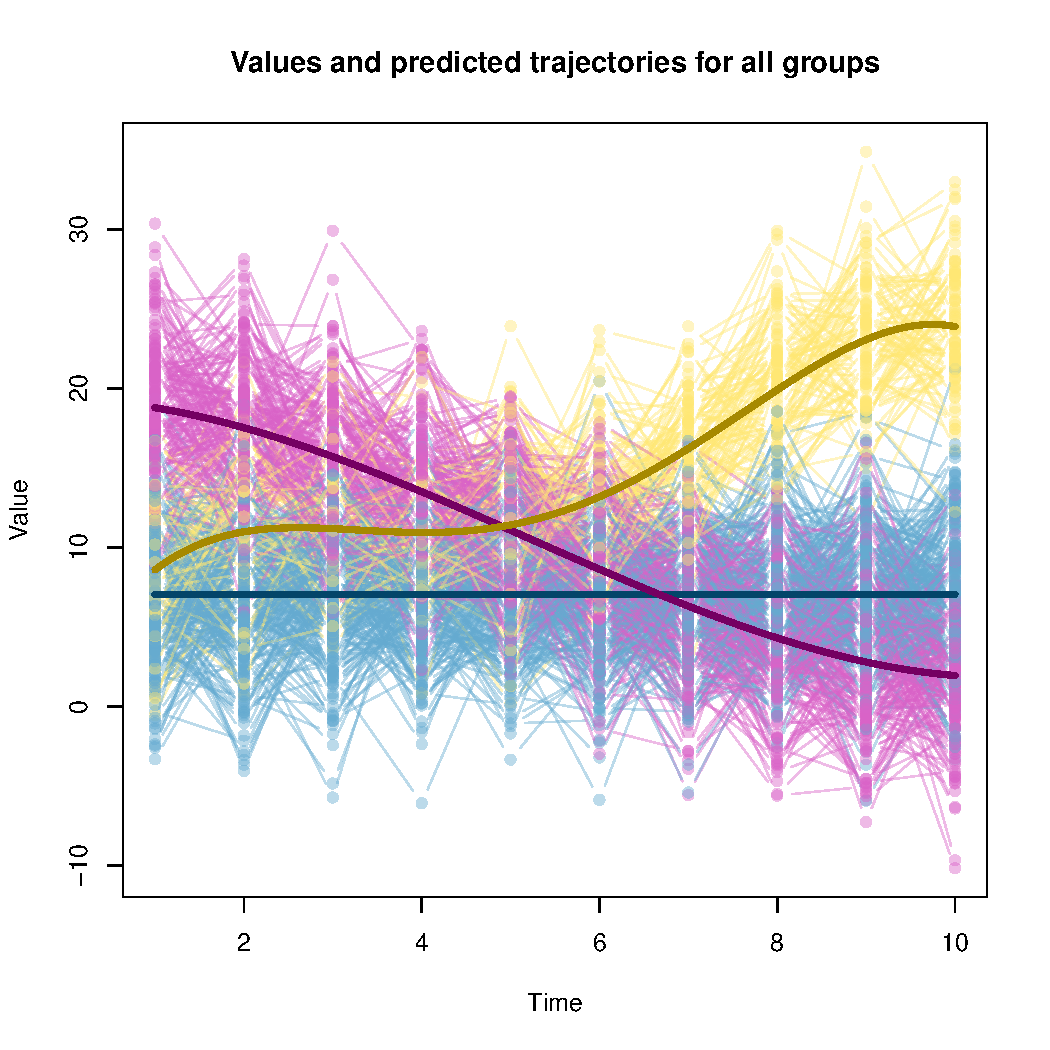
\includegraphics[width=\maxwidth]{figure/unnamed-chunk-28-1} 

\end{knitrout}

\subsection{Adding covariate}
In the same way that in the section below we can add covariate in the calculus of the parameters with or without option same sigma. \\

If we add risk variable we use option \verb|Risk =|.
\begin{knitrout}
\definecolor{shadecolor}{rgb}{0.969, 0.969, 0.969}\color{fgcolor}\begin{kframe}
\begin{alltt}
\hlstd{solLRisks} \hlkwb{=} \hlkwd{trajeR}\hlstd{(}\hlkwc{Y} \hlstd{= data[,}\hlnum{2}\hlopt{:}\hlnum{11}\hlstd{],} \hlkwc{A} \hlstd{= data[,}\hlnum{12}\hlopt{:}\hlnum{21}\hlstd{],} \hlkwc{Risk} \hlstd{= data[,}\hlnum{42}\hlopt{:}\hlnum{43}\hlstd{],}
                   \hlkwc{ng} \hlstd{=} \hlnum{3}\hlstd{,} \hlkwc{degre} \hlstd{=} \hlkwd{c}\hlstd{(}\hlnum{0}\hlstd{,}\hlnum{3}\hlstd{,}\hlnum{4}\hlstd{),}
                   \hlkwc{Model} \hlstd{=} \hlstr{"CNORM"}\hlstd{,} \hlkwc{Method} \hlstd{=} \hlstr{"L"}\hlstd{,} \hlkwc{ssigma} \hlstd{=} \hlnum{TRUE}\hlstd{,} \hlkwc{hessian} \hlstd{=} \hlnum{FALSE}\hlstd{)}
\end{alltt}
\end{kframe}
\end{knitrout}
\begin{knitrout}
\definecolor{shadecolor}{rgb}{0.969, 0.969, 0.969}\color{fgcolor}\begin{kframe}
\begin{alltt}
\hlstd{solLRisks}
\end{alltt}
\begin{verbatim}
## Call TrajeR with 3 groups and a 0,3,4 degrees of polynomial shape of trajectory.
## Model : Censored Normal
## Method : Likelihood 
##  
##   group   Parameter   Estimate   Std. Error   T for H0:   Prob>|T|  
##                                                param.=0             
## --------------------------------------------------------------------
##       1   Intercept    7.05305      0.04176   168.90808          0  
##                                                                     
##       2   Intercept   19.31485      0.11614   166.30125          0  
##              Linear   -0.09043      0.11968    -0.75564     0.4499  
##           Quadratic   -0.45729      0.04884    -9.36403          0  
##               Cubic    0.02926      0.03016      0.9701    0.33204  
##                                                                     
##       3   Intercept    1.66973      0.03157     52.8925          0  
##              Linear   10.11813      0.08516   118.81332          0  
##           Quadratic   -3.70714      0.07949   -46.63367          0  
##               Cubic    0.53762      0.10117     5.31376          0  
##             Quartic   -0.02459      0.03642    -0.67503    0.49969  
## --------------------------------------------------------------------
##       1      sigma1    4.02023      0.00277   1450.09467          0  
##       2      sigma2    4.02023      0.01226    327.8234          0  
##       3      sigma3    4.02023      0.02714    148.1213          0  
## --------------------------------------------------------------------
##       1    Baseline          0      0.04392    36.76149          0  
##                                                                     
##       2   Intercept   -0.65926          NaN         NaN        NaN  
##                 V42    0.19556      0.01854    59.05037          0  
##                 V43    0.57349          NaN         NaN        NaN  
##                                                                     
##       3   Intercept   -1.18455       0.0403     10.6709          0  
##                 V42    0.10637      0.13123     7.66374          0  
##                 V43    0.52564      0.13637      8.5007          0  
## --------------------------------------------------------------------
## Likelihood : -14563.99
\end{verbatim}
\end{kframe}
\end{knitrout}


\begin{table}[H]
\centering
\begin{tabular}{rrrr}
\toprule
\multicolumn{2}{c}{Different sigma} & \multicolumn{2}{c}{Same sigma} \\
\cmidrule(l{3pt}r{3pt}){1-2} \cmidrule(l{3pt}r{3pt}){3-4}
SolLRisk & SolEMRisk & SolLRisks & SolEMRisks\\
\midrule
\addlinespace[0.3em]
\multicolumn{4}{l}{\textbf{Beta 1}}\\
\hspace{1em}7.04921 & 7.05035 & 7.05305 & 7.05409\\
\addlinespace[0.3em]
\multicolumn{4}{l}{\textbf{Beta 2}}\\
\hspace{1em}19.30527 & 19.30744 & 19.31485 & 19.31750\\
\hspace{1em}-0.09488 & -0.09202 & -0.09043 & -0.08838\\
\hspace{1em}-0.45575 & -0.45655 & -0.45729 & -0.45791\\
\hspace{1em}0.02917 & 0.02922 & 0.02926 & 0.02930\\
\addlinespace[0.3em]
\multicolumn{4}{l}{\textbf{Beta 3}}\\
\hspace{1em}1.68068 & 1.66949 & 1.66973 & 1.66950\\
\hspace{1em}10.10606 & 10.11832 & 10.11813 & 10.11839\\
\hspace{1em}-3.70319 & -3.70726 & -3.70714 & -3.70727\\
\hspace{1em}0.53712 & 0.53764 & 0.53762 & 0.53764\\
\hspace{1em}-0.02456 & -0.02459 & -0.02459 & -0.02459\\
\addlinespace[0.3em]
\multicolumn{4}{l}{\textbf{Sigma}}\\
\hspace{1em}3.95758 & 3.95861 & 4.02023 & 4.02028\\
\hspace{1em}4.11102 & 4.11005 & 4.02023 & 4.02028\\
\hspace{1em}4.00154 & 4.00167 & 4.02023 & 4.02028\\
\addlinespace[0.3em]
\multicolumn{4}{l}{\textbf{Theta - First group 0}}\\
\hspace{1em}-0.65610 & -0.65362 & -0.65926 & -0.65664\\
\hspace{1em}0.19568 & 0.19586 & 0.19556 & 0.19540\\
\hspace{1em}0.57614 & 0.56777 & 0.57349 & 0.56554\\
\hspace{1em}-1.18333 & -1.18219 & -1.18455 & -1.18317\\
\hspace{1em}0.10695 & 0.10703 & 0.10637 & 0.10649\\
\hspace{1em}0.52682 & 0.52299 & 0.52564 & 0.52157\\
\bottomrule
\end{tabular}
\end{table}



If we add time dependent covariate we use option \verb|TCOV|.
\begin{knitrout}
\definecolor{shadecolor}{rgb}{0.969, 0.969, 0.969}\color{fgcolor}\begin{kframe}
\begin{alltt}
\hlstd{solLTCOV2} \hlkwb{=} \hlkwd{trajeR}\hlstd{(}\hlkwc{Y} \hlstd{= data[,}\hlnum{2}\hlopt{:}\hlnum{11}\hlstd{],} \hlkwc{A} \hlstd{= data[,}\hlnum{12}\hlopt{:}\hlnum{21}\hlstd{],} \hlkwc{TCOV} \hlstd{= data[,}\hlnum{22}\hlopt{:}\hlnum{41}\hlstd{],}
                   \hlkwc{ng} \hlstd{=} \hlnum{3}\hlstd{,} \hlkwc{degre} \hlstd{=} \hlkwd{c}\hlstd{(}\hlnum{0}\hlstd{,}\hlnum{3}\hlstd{,}\hlnum{4}\hlstd{),}
                   \hlkwc{Model} \hlstd{=} \hlstr{"CNORM"}\hlstd{,} \hlkwc{Method} \hlstd{=} \hlstr{"L"}\hlstd{,} \hlkwc{ssigma} \hlstd{=} \hlnum{FALSE}\hlstd{,} \hlkwc{hessian} \hlstd{=} \hlnum{FALSE}\hlstd{)}
\end{alltt}
\end{kframe}
\end{knitrout}
\begin{knitrout}
\definecolor{shadecolor}{rgb}{0.969, 0.969, 0.969}\color{fgcolor}\begin{kframe}
\begin{alltt}
\hlstd{solLTCOV2}
\end{alltt}
\begin{verbatim}
## Call TrajeR with 3 groups and a 0,3,4 degrees of polynomial shape of trajectory.
## Model : Censored Normal
## Method : Likelihood 
##  
##   group   Parameter   Estimate   Std. Error   T for H0:   Prob>|T|  
##                                                param.=0             
## --------------------------------------------------------------------
##       1   Intercept    6.75745      0.08309    81.32696          0  
##               TCOV1   -0.00358      0.16289    -0.02195    0.98249  
##               TCOV2    0.58151      0.06557     8.86839          0  
##                                                                     
##       2   Intercept   19.45552      0.07795   249.59559          0  
##              Linear   -0.09592      0.10136    -0.94628    0.34405  
##           Quadratic   -0.45507      0.03622   -12.56502          0  
##               Cubic     0.0291      0.00277    10.51302          0  
##               TCOV1   -0.17051      0.19635     -0.8684    0.38522  
##               TCOV2   -0.13303      0.05521    -2.40954    0.01601  
##                                                                     
##       3   Intercept    1.79828      0.06183    29.08577          0  
##              Linear   10.13362      0.03745   270.57751          0  
##           Quadratic   -3.71451      0.07286   -50.98126          0  
##               Cubic    0.53887      0.01732    31.10904          0  
##             Quartic   -0.02465      0.00106   -23.18069          0  
##               TCOV1    0.08064      0.21207     0.38024    0.70378  
##               TCOV2    -0.3598        0.038    -9.46729          0  
## --------------------------------------------------------------------
##       1      sigma1    3.95415      0.01531   258.26618          0  
##       2      sigma2    4.10997      0.01714   239.80629          0  
##       3      sigma3    4.00024      0.02353   169.98647          0  
## --------------------------------------------------------------------
##       1         pi1    0.45881       0.0617    22.38634          0  
##       2         pi2    0.34911      0.06516    17.00593          0  
##       3         pi3    0.19207       0.0761     6.70953          0  
## --------------------------------------------------------------------
## Likelihood : -14561.48
\end{verbatim}
\end{kframe}
\end{knitrout}
Here we can use all method and with or without same sigma.
\begin{knitrout}
\definecolor{shadecolor}{rgb}{0.969, 0.969, 0.969}\color{fgcolor}\begin{kframe}
\begin{alltt}
\hlstd{solLTCOV2s} \hlkwb{=} \hlkwd{trajeR}\hlstd{(data[,}\hlnum{2}\hlopt{:}\hlnum{11}\hlstd{], data[,}\hlnum{12}\hlopt{:}\hlnum{21}\hlstd{],} \hlkwc{TCOV} \hlstd{= data[,}\hlnum{22}\hlopt{:}\hlnum{41}\hlstd{],} \hlkwc{ng} \hlstd{=} \hlnum{3}\hlstd{,} \hlkwc{degre}\hlstd{=}\hlkwd{c}\hlstd{(}\hlnum{0}\hlstd{,}\hlnum{3}\hlstd{,}\hlnum{4}\hlstd{),}
                   \hlkwc{Model}\hlstd{=}\hlstr{"CNORM"}\hlstd{,} \hlkwc{Method} \hlstd{=} \hlstr{"L"}\hlstd{,} \hlkwc{ssigma} \hlstd{=} \hlnum{TRUE}\hlstd{,} \hlkwc{hessian} \hlstd{=} \hlnum{FALSE}\hlstd{)}
\hlstd{solEMTCOV2} \hlkwb{=} \hlkwd{trajeR}\hlstd{(data[,}\hlnum{2}\hlopt{:}\hlnum{11}\hlstd{], data[,}\hlnum{12}\hlopt{:}\hlnum{21}\hlstd{],} \hlkwc{TCOV} \hlstd{= data[,}\hlnum{22}\hlopt{:}\hlnum{41}\hlstd{],} \hlkwc{ng} \hlstd{=} \hlnum{3}\hlstd{,} \hlkwc{degre}\hlstd{=}\hlkwd{c}\hlstd{(}\hlnum{0}\hlstd{,}\hlnum{3}\hlstd{,}\hlnum{4}\hlstd{),}
                  \hlkwc{Model}\hlstd{=}\hlstr{"CNORM"}\hlstd{,} \hlkwc{Method} \hlstd{=} \hlstr{"EM"}\hlstd{,} \hlkwc{ssigma} \hlstd{=} \hlnum{FALSE}\hlstd{,} \hlkwc{hessian} \hlstd{=} \hlnum{FALSE}\hlstd{)}
\hlstd{solEMTCOV2s} \hlkwb{=} \hlkwd{trajeR}\hlstd{(data[,}\hlnum{2}\hlopt{:}\hlnum{11}\hlstd{], data[,}\hlnum{12}\hlopt{:}\hlnum{21}\hlstd{],} \hlkwc{TCOV} \hlstd{= data[,}\hlnum{22}\hlopt{:}\hlnum{41}\hlstd{],} \hlkwc{ng} \hlstd{=} \hlnum{3}\hlstd{,} \hlkwc{degre}\hlstd{=}\hlkwd{c}\hlstd{(}\hlnum{0}\hlstd{,}\hlnum{3}\hlstd{,}\hlnum{4}\hlstd{),}
                  \hlkwc{Model}\hlstd{=}\hlstr{"CNORM"}\hlstd{,} \hlkwc{Method} \hlstd{=} \hlstr{"EM"}\hlstd{,} \hlkwc{ssigma} \hlstd{=} \hlnum{TRUE}\hlstd{,} \hlkwc{hessian} \hlstd{=} \hlnum{FALSE}\hlstd{)}
\end{alltt}
\end{kframe}
\end{knitrout}
We have

\begin{table}[H]
\centering
\begin{tabular}{rrrr}
\toprule
\multicolumn{2}{c}{Different sigma} & \multicolumn{2}{c}{Same sigma} \\
\cmidrule(l{3pt}r{3pt}){1-2} \cmidrule(l{3pt}r{3pt}){3-4}
SolLTCOV2 & SolEMCOV2 & SolLTCOV2s & SolEMCOV2s\\
\midrule
\addlinespace[0.3em]
\multicolumn{4}{l}{\textbf{Beta 1}}\\
\hspace{1em}6.75745 & 6.75763 & 6.76374 & 6.76375\\
\addlinespace[0.3em]
\multicolumn{4}{l}{\textbf{Beta 2}}\\
\hspace{1em}19.45552 & 19.45636 & 19.46899 & 19.46852\\
\hspace{1em}-0.09592 & -0.09667 & -0.09357 & -0.09328\\
\hspace{1em}-0.45507 & -0.45490 & -0.45619 & -0.45624\\
\hspace{1em}0.02910 & 0.02909 & 0.02917 & 0.02917\\
\addlinespace[0.3em]
\multicolumn{4}{l}{\textbf{Beta 3}}\\
\hspace{1em}1.79828 & 1.81447 & 1.81399 & 1.81446\\
\hspace{1em}10.13362 & 10.11476 & 10.11540 & 10.11485\\
\hspace{1em}-3.71451 & -3.70808 & -3.70827 & -3.70809\\
\hspace{1em}0.53887 & 0.53803 & 0.53806 & 0.53803\\
\hspace{1em}-0.02465 & -0.02462 & -0.02462 & -0.02462\\
\addlinespace[0.3em]
\multicolumn{4}{l}{\textbf{Sigma}}\\
\hspace{1em}3.95415 & 3.95414 & 4.01798 & 4.01801\\
\hspace{1em}4.10997 & 4.11016 & 4.01798 & 4.01801\\
\hspace{1em}4.00024 & 4.00019 & 4.01798 & 4.01801\\
\addlinespace[0.3em]
\multicolumn{4}{l}{\textbf{Delta 1}}\\
\hspace{1em}-0.00358 & -0.00354 & -0.00768 & -0.00762\\
\hspace{1em}0.58151 & 0.58136 & 0.58100 & 0.58095\\
\addlinespace[0.3em]
\multicolumn{4}{l}{\textbf{Delta 2}}\\
\hspace{1em}-0.17051 & -0.17068 & -0.16727 & -0.16724\\
\hspace{1em}-0.13303 & -0.13289 & -0.13786 & -0.13777\\
\addlinespace[0.3em]
\multicolumn{4}{l}{\textbf{Delta 3}}\\
\hspace{1em}0.08064 & 0.08049 & 0.08040 & 0.08044\\
\hspace{1em}-0.35980 & -0.35939 & -0.35958 & -0.35934\\
\addlinespace[0.3em]
\multicolumn{4}{l}{\textbf{Pi}}\\
\hspace{1em}0.45881 & 0.45879 & 0.45968 & 0.45970\\
\hspace{1em}0.34911 & 0.34913 & 0.34824 & 0.34823\\
\hspace{1em}0.19207 & 0.19208 & 0.19208 & 0.19207\\
\bottomrule
\end{tabular}
\end{table}



\section{Censored Data}

We have modified the previous data are such way that they become censored data. All values upper to 23 become 233 and  those smaller to 2 become 2.\\
So we obtained data that follow a censored normal distribution. If we don't take into consideration this fact,
\begin{knitrout}
\definecolor{shadecolor}{rgb}{0.969, 0.969, 0.969}\color{fgcolor}\begin{kframe}
\begin{alltt}
\hlstd{solLC} \hlkwb{=} \hlkwd{trajeR}\hlstd{(}\hlkwc{Y} \hlstd{= dataC[,}\hlnum{2}\hlopt{:}\hlnum{11}\hlstd{],} \hlkwc{A} \hlstd{= dataC[,}\hlnum{12}\hlopt{:}\hlnum{21}\hlstd{],}
               \hlkwc{ng} \hlstd{=} \hlnum{3}\hlstd{,} \hlkwc{degre} \hlstd{=} \hlkwd{c}\hlstd{(}\hlnum{0}\hlstd{,}\hlnum{3}\hlstd{,}\hlnum{4}\hlstd{),}
               \hlkwc{Model}\hlstd{=}\hlstr{"CNORM"}\hlstd{,} \hlkwc{Method} \hlstd{=} \hlstr{"L"}\hlstd{,} \hlkwc{ssigma} \hlstd{=} \hlnum{FALSE}\hlstd{,} \hlkwc{hessian} \hlstd{=} \hlnum{FALSE}\hlstd{,}
               \hlkwc{ymin}\hlstd{=}\hlnum{2}\hlstd{,} \hlkwc{ymax}\hlstd{=}\hlnum{23}\hlstd{)}
\end{alltt}
\end{kframe}
\end{knitrout}
\begin{knitrout}
\definecolor{shadecolor}{rgb}{0.969, 0.969, 0.969}\color{fgcolor}\begin{kframe}
\begin{alltt}
\hlstd{solLC}
\end{alltt}
\begin{verbatim}
## Call TrajeR with 3 groups and a 0,3,4 degrees of polynomial shape of trajectory.
## Model : Censored Normal
## Method : Likelihood 
##  
##   group   Parameter   Estimate   Std. Error   T for H0:   Prob>|T|  
##                                                param.=0             
## --------------------------------------------------------------------
##       1   Intercept    7.06349      0.08309    85.01078          0  
##                                                                     
##       2   Intercept   19.22938      0.08478   226.81088          0  
##              Linear   -0.08816      0.10743    -0.82057    0.41193  
##           Quadratic   -0.44944      0.03883   -11.57498          0  
##               Cubic    0.02842      0.00297     9.58168          0  
##                                                                     
##       3   Intercept    1.46919       0.0892    16.46982          0  
##              Linear   10.30385      0.12286    83.86753          0  
##           Quadratic   -3.76773          NaN         NaN        NaN  
##               Cubic    0.54588          NaN         NaN        NaN  
##             Quartic   -0.02499          NaN         NaN        NaN  
## --------------------------------------------------------------------
##       1      sigma1     3.9223      0.01609   243.72812          0  
##       2      sigma2    4.10489      0.01955    209.9628          0  
##       3      sigma3    4.00575      0.00694   576.81651          0  
## --------------------------------------------------------------------
##       1         pi1    0.45833       0.0614    22.47794          0  
##       2         pi2    0.34959      0.06512    17.03599          0  
##       3         pi3    0.19209      0.07573     6.74124          0  
## --------------------------------------------------------------------
## Likelihood : -13317.83
\end{verbatim}
\begin{alltt}
\hlkwd{plot}\hlstd{(solLC,} \hlkwc{Y} \hlstd{= dataC[,}\hlnum{2}\hlopt{:}\hlnum{11}\hlstd{],} \hlkwc{A} \hlstd{= dataC[,}\hlnum{12}\hlopt{:}\hlnum{21}\hlstd{],} \hlkwc{col} \hlstd{= vcol)}
\end{alltt}
\end{kframe}
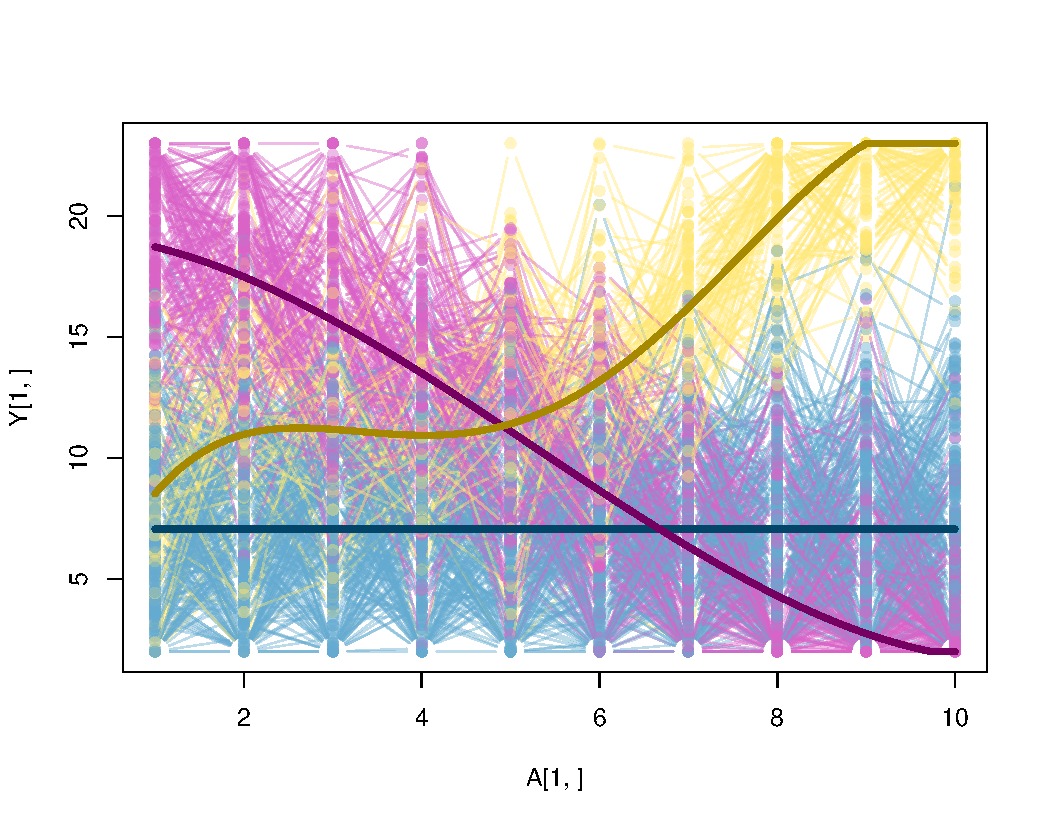
\includegraphics[width=\maxwidth]{figure/unnamed-chunk-39-1} 

\end{knitrout}
If we surch the solution without consider the fact that the data are not censored, we find parameters that are wrong. They considere that the max and min are really max and min while the real values are omitted. To illustrate this fact we compute the paramters without censored.

\begin{table}[H]
\centering
\begin{tabular}{rr}
\toprule
Censored & Not Censored\\
\midrule
\addlinespace[0.3em]
\multicolumn{2}{l}{\textbf{Beta 1}}\\
\hspace{1em}7.0634900 & 7.2424800\\
\addlinespace[0.3em]
\multicolumn{2}{l}{\textbf{Beta 2}}\\
\hspace{1em}19.2293800 & 18.8466500\\
\hspace{1em}-0.0881600 & 0.0639900\\
\hspace{1em}-0.4494400 & -0.4835500\\
\hspace{1em}0.0284200 & 0.0324500\\
\addlinespace[0.3em]
\multicolumn{2}{l}{\textbf{Beta 3}}\\
\hspace{1em}1.4691900 & 2.3253200\\
\hspace{1em}10.3038500 & 9.3139500\\
\hspace{1em}-3.7677300 & -3.4181600\\
\hspace{1em}0.5458800 & 0.5013300\\
\hspace{1em}-0.0249900 & -0.0233200\\
\addlinespace[0.3em]
\multicolumn{2}{l}{\textbf{Sigma}}\\
\hspace{1em}3.9223000 & 3.5980600\\
\hspace{1em}4.1048900 & 3.5482400\\
\hspace{1em}4.0057500 & 3.6012300\\
\addlinespace[0.3em]
\multicolumn{2}{l}{\textbf{Pi}}\\
\hspace{1em}0.4583245 & 0.4588787\\
\hspace{1em}0.3495887 & 0.3489176\\
\hspace{1em}0.1920868 & 0.1922037\\
\bottomrule
\end{tabular}
\end{table}


We cans ee the difference between the two situation in the graphics above. The right one is calculted by considering censored data and it is close to the right solution and the trajectory consider the missing values by continuing up while the second considere the max and min like real value and the trajectory is smaller.
\begin{knitrout}
\definecolor{shadecolor}{rgb}{0.969, 0.969, 0.969}\color{fgcolor}\begin{kframe}
\begin{alltt}
\hlkwd{par}\hlstd{(}\hlkwc{mfrow}\hlstd{=}\hlkwd{c}\hlstd{(}\hlnum{1}\hlstd{,}\hlnum{2}\hlstd{))}
\hlkwd{plot}\hlstd{(solLC,} \hlkwc{Y} \hlstd{= dataC[,}\hlnum{2}\hlopt{:}\hlnum{11}\hlstd{],} \hlkwc{A} \hlstd{= dataC[,}\hlnum{12}\hlopt{:}\hlnum{21}\hlstd{],} \hlkwc{col} \hlstd{= vcol,} \hlkwc{main}\hlstd{=}\hlstr{"Censored"}\hlstd{)}
\hlkwd{plot}\hlstd{(solLnC,} \hlkwc{Y} \hlstd{= dataC[,}\hlnum{2}\hlopt{:}\hlnum{11}\hlstd{],} \hlkwc{A} \hlstd{= dataC[,}\hlnum{12}\hlopt{:}\hlnum{21}\hlstd{],} \hlkwc{col} \hlstd{= vcol,} \hlkwc{main}\hlstd{=}\hlstr{"Not Censored"} \hlstd{)}
\end{alltt}
\end{kframe}
\end{knitrout}
\hspace*{-3.5cm}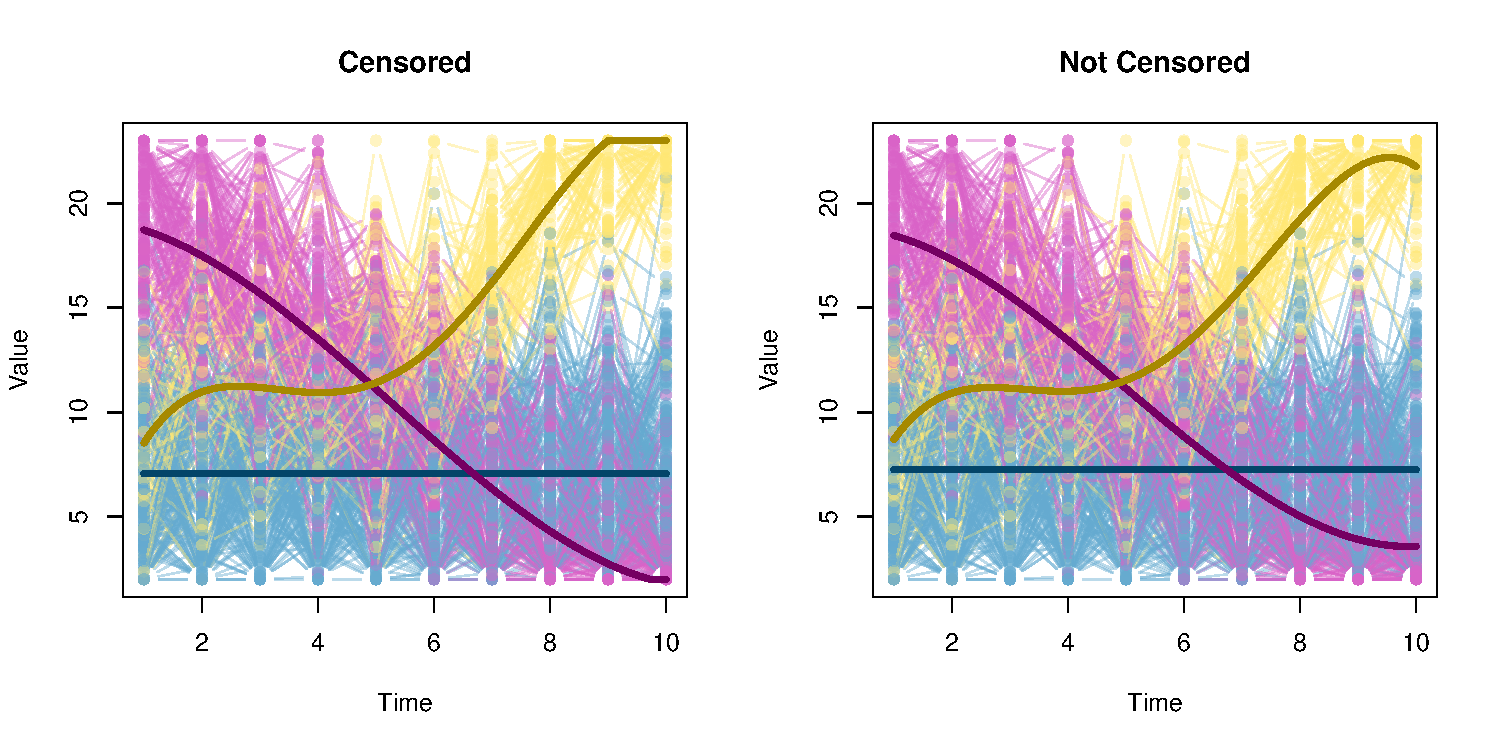
\includegraphics[scale=0.8]{figure/generate_figures-1}
For all the method we have
\begin{knitrout}
\definecolor{shadecolor}{rgb}{0.969, 0.969, 0.969}\color{fgcolor}\begin{kframe}
\begin{alltt}
\hlstd{solLCs} \hlkwb{=} \hlkwd{trajeR}\hlstd{(}\hlkwc{Y} \hlstd{= data[,}\hlnum{2}\hlopt{:}\hlnum{11}\hlstd{],} \hlkwc{A} \hlstd{= data[,}\hlnum{12}\hlopt{:}\hlnum{21}\hlstd{],}
                \hlkwc{ng} \hlstd{=} \hlnum{3}\hlstd{,} \hlkwc{degre} \hlstd{=} \hlkwd{c}\hlstd{(}\hlnum{0}\hlstd{,}\hlnum{3}\hlstd{,}\hlnum{4}\hlstd{),}
                \hlkwc{Model}\hlstd{=}\hlstr{"CNORM"}\hlstd{,} \hlkwc{Method} \hlstd{=} \hlstr{"L"}\hlstd{,} \hlkwc{ssigma} \hlstd{=} \hlnum{TRUE}\hlstd{,} \hlkwc{hessian} \hlstd{=} \hlnum{FALSE}\hlstd{,}
                \hlkwc{ymin} \hlstd{=} \hlnum{2}\hlstd{,}  \hlkwc{ymax} \hlstd{=} \hlnum{23}\hlstd{)}
\hlstd{solEMC} \hlkwb{=} \hlkwd{trajeR}\hlstd{(}\hlkwc{Y} \hlstd{= data[,}\hlnum{2}\hlopt{:}\hlnum{11}\hlstd{],} \hlkwc{A} \hlstd{= data[,}\hlnum{12}\hlopt{:}\hlnum{21}\hlstd{],}
                \hlkwc{ng} \hlstd{=} \hlnum{3}\hlstd{,} \hlkwc{degre} \hlstd{=} \hlkwd{c}\hlstd{(}\hlnum{0}\hlstd{,}\hlnum{3}\hlstd{,}\hlnum{4}\hlstd{),}
                \hlkwc{Model}\hlstd{=}\hlstr{"CNORM"}\hlstd{,} \hlkwc{Method} \hlstd{=} \hlstr{"EM"}\hlstd{,} \hlkwc{ssigma} \hlstd{=} \hlnum{FALSE}\hlstd{,} \hlkwc{hessian} \hlstd{=} \hlnum{FALSE}\hlstd{,}
                \hlkwc{ymin} \hlstd{=} \hlnum{2}\hlstd{,}  \hlkwc{ymax} \hlstd{=} \hlnum{23}\hlstd{)}
\hlstd{solEMnC} \hlkwb{=} \hlkwd{trajeR}\hlstd{(}\hlkwc{Y} \hlstd{= data[,}\hlnum{2}\hlopt{:}\hlnum{11}\hlstd{],} \hlkwc{A} \hlstd{= data[,}\hlnum{12}\hlopt{:}\hlnum{21}\hlstd{],}
                 \hlkwc{ng} \hlstd{=} \hlnum{3}\hlstd{,} \hlkwc{degre} \hlstd{=} \hlkwd{c}\hlstd{(}\hlnum{0}\hlstd{,}\hlnum{3}\hlstd{,}\hlnum{4}\hlstd{),}
                 \hlkwc{Model}\hlstd{=}\hlstr{"CNORM"}\hlstd{,} \hlkwc{Method} \hlstd{=} \hlstr{"EM"}\hlstd{,} \hlkwc{ssigma} \hlstd{=} \hlnum{FALSE}\hlstd{,} \hlkwc{hessian} \hlstd{=} \hlnum{FALSE}\hlstd{)}
\end{alltt}
\end{kframe}
\end{knitrout}

\begin{table}[H]
\centering
\begin{tabular}{rrrr}
\toprule
\multicolumn{2}{c}{Different sigma} & \multicolumn{2}{c}{Same sigma} \\
\cmidrule(l{3pt}r{3pt}){1-2} \cmidrule(l{3pt}r{3pt}){3-4}
SolLC & SolEMC & SolLCs & SolEMCs\\
\midrule
\addlinespace[0.3em]
\multicolumn{4}{l}{\textbf{Beta 1}}\\
\hspace{1em}7.06349 & 7.06352 & 7.06263 & 7.06261\\
\addlinespace[0.3em]
\multicolumn{4}{l}{\textbf{Beta 2}}\\
\hspace{1em}19.22938 & 19.23116 & 19.22999 & 19.23109\\
\hspace{1em}-0.08816 & -0.08916 & -0.08092 & -0.08164\\
\hspace{1em}-0.44944 & -0.44929 & -0.45150 & -0.45135\\
\hspace{1em}0.02842 & 0.02841 & 0.02860 & 0.02859\\
\addlinespace[0.3em]
\multicolumn{4}{l}{\textbf{Beta 3}}\\
\hspace{1em}1.46919 & 1.47075 & 1.47182 & 1.47257\\
\hspace{1em}10.30385 & 10.30213 & 10.30113 & 10.30028\\
\hspace{1em}-3.76773 & -3.76720 & -3.76673 & -3.76648\\
\hspace{1em}0.54588 & 0.54581 & 0.54574 & 0.54571\\
\hspace{1em}-0.02499 & -0.02499 & -0.02498 & -0.02498\\
\addlinespace[0.3em]
\multicolumn{4}{l}{\textbf{Sigma}}\\
\hspace{1em}3.92230 & 3.92236 & 3.99933 & 3.99933\\
\hspace{1em}4.10489 & 4.10491 & 3.99933 & 3.99933\\
\hspace{1em}4.00575 & 4.00573 & 3.99933 & 3.99933\\
\addlinespace[0.3em]
\multicolumn{4}{l}{\textbf{Pi}}\\
\hspace{1em}0.45833 & 0.45829 & 0.45939 & 0.45937\\
\hspace{1em}0.34959 & 0.34961 & 0.34855 & 0.34855\\
\hspace{1em}0.19209 & 0.19210 & 0.19207 & 0.19208\\
\bottomrule
\end{tabular}
\end{table}



We can add time covariate to the censored data.
\begin{knitrout}
\definecolor{shadecolor}{rgb}{0.969, 0.969, 0.969}\color{fgcolor}\begin{kframe}
\begin{alltt}
\hlstd{solLCTCOV} \hlkwb{=} \hlkwd{trajeR}\hlstd{(}\hlkwc{Y} \hlstd{= data[,}\hlnum{2}\hlopt{:}\hlnum{11}\hlstd{],} \hlkwc{A} \hlstd{= data[,}\hlnum{12}\hlopt{:}\hlnum{21}\hlstd{],} \hlkwc{TCOV} \hlstd{= data[,}\hlnum{22}\hlopt{:}\hlnum{31}\hlstd{],}
                   \hlkwc{ng} \hlstd{=} \hlnum{3}\hlstd{,} \hlkwc{degre} \hlstd{=} \hlkwd{c}\hlstd{(}\hlnum{0}\hlstd{,}\hlnum{3}\hlstd{,}\hlnum{4}\hlstd{),}
                   \hlkwc{Model} \hlstd{=} \hlstr{"CNORM"}\hlstd{,} \hlkwc{Method} \hlstd{=} \hlstr{"L"}\hlstd{,} \hlkwc{ssigma} \hlstd{=} \hlnum{FALSE}\hlstd{,} \hlkwc{hessian} \hlstd{=} \hlnum{FALSE}\hlstd{,}
                   \hlkwc{ymin} \hlstd{=} \hlnum{2}\hlstd{,}  \hlkwc{ymax} \hlstd{=} \hlnum{23}\hlstd{)}
\hlstd{solLCTCOVs} \hlkwb{=} \hlkwd{trajeR}\hlstd{(}\hlkwc{Y} \hlstd{= data[,}\hlnum{2}\hlopt{:}\hlnum{11}\hlstd{],} \hlkwc{A} \hlstd{= data[,}\hlnum{12}\hlopt{:}\hlnum{21}\hlstd{],} \hlkwc{TCOV} \hlstd{= data[,}\hlnum{22}\hlopt{:}\hlnum{31}\hlstd{],}
                    \hlkwc{ng} \hlstd{=} \hlnum{3}\hlstd{,} \hlkwc{degre} \hlstd{=} \hlkwd{c}\hlstd{(}\hlnum{0}\hlstd{,}\hlnum{3}\hlstd{,}\hlnum{4}\hlstd{),}
                    \hlkwc{Model} \hlstd{=} \hlstr{"CNORM"}\hlstd{,} \hlkwc{Method} \hlstd{=} \hlstr{"L"}\hlstd{,} \hlkwc{ssigma} \hlstd{=} \hlnum{TRUE}\hlstd{,} \hlkwc{hessian} \hlstd{=} \hlnum{FALSE}\hlstd{,}
                    \hlkwc{ymin} \hlstd{=} \hlnum{2}\hlstd{,}  \hlkwc{ymax} \hlstd{=} \hlnum{23}\hlstd{)}
\hlstd{solEMCTCOV} \hlkwb{=} \hlkwd{trajeR}\hlstd{(}\hlkwc{Y} \hlstd{= data[,}\hlnum{2}\hlopt{:}\hlnum{11}\hlstd{],} \hlkwc{A} \hlstd{= data[,}\hlnum{12}\hlopt{:}\hlnum{21}\hlstd{],} \hlkwc{TCOV} \hlstd{= data[,}\hlnum{22}\hlopt{:}\hlnum{31}\hlstd{],}
                    \hlkwc{ng} \hlstd{=} \hlnum{3}\hlstd{,} \hlkwc{degre} \hlstd{=} \hlkwd{c}\hlstd{(}\hlnum{0}\hlstd{,}\hlnum{3}\hlstd{,}\hlnum{4}\hlstd{),}
                    \hlkwc{Model} \hlstd{=} \hlstr{"CNORM"}\hlstd{,} \hlkwc{Method} \hlstd{=} \hlstr{"EM"}\hlstd{,} \hlkwc{ssigma} \hlstd{=} \hlnum{TRUE}\hlstd{,} \hlkwc{hessian} \hlstd{=} \hlnum{FALSE}\hlstd{,}
                    \hlkwc{ymin} \hlstd{=} \hlnum{2}\hlstd{,}  \hlkwc{ymax} \hlstd{=} \hlnum{23}\hlstd{)}
\hlstd{solEMCTCOVs} \hlkwb{=} \hlkwd{trajeR}\hlstd{(}\hlkwc{Y} \hlstd{= data[,}\hlnum{2}\hlopt{:}\hlnum{11}\hlstd{],} \hlkwc{A} \hlstd{= data[,}\hlnum{12}\hlopt{:}\hlnum{21}\hlstd{],} \hlkwc{TCOV} \hlstd{= data[,}\hlnum{22}\hlopt{:}\hlnum{31}\hlstd{],}
                     \hlkwc{ng} \hlstd{=} \hlnum{3}\hlstd{,} \hlkwc{degre} \hlstd{=} \hlkwd{c}\hlstd{(}\hlnum{0}\hlstd{,}\hlnum{3}\hlstd{,}\hlnum{4}\hlstd{),}
                     \hlkwc{Model} \hlstd{=} \hlstr{"CNORM"}\hlstd{,} \hlkwc{Method} \hlstd{=} \hlstr{"EM"}\hlstd{,} \hlkwc{ssigma} \hlstd{=} \hlnum{FALSE}\hlstd{,} \hlkwc{hessian} \hlstd{=} \hlnum{FALSE}\hlstd{,}
                     \hlkwc{ymin} \hlstd{=} \hlnum{2}\hlstd{,}  \hlkwc{ymax} \hlstd{=} \hlnum{23}\hlstd{)}
\end{alltt}
\end{kframe}
\end{knitrout}

\begin{table}[H]
\centering
\begin{tabular}{rrrr}
\toprule
\multicolumn{2}{c}{Different sigma} & \multicolumn{2}{c}{Same sigma} \\
\cmidrule(l{3pt}r{3pt}){1-2} \cmidrule(l{3pt}r{3pt}){3-4}
SolLCTCOV & SolEMCTCOV & SolLCTCOVs & SolEMCTCOVs\\
\midrule
\addlinespace[0.3em]
\multicolumn{4}{l}{\textbf{Beta 1}}\\
\hspace{1em}7.05896 & 7.06301 & 7.06096 & 7.06103\\
\addlinespace[0.3em]
\multicolumn{4}{l}{\textbf{Beta 2}}\\
\hspace{1em}19.32135 & 19.22625 & 19.31753 & 19.31862\\
\hspace{1em}-0.08348 & -0.08963 & -0.07488 & -0.07567\\
\hspace{1em}-0.44995 & -0.44880 & -0.45224 & -0.45206\\
\hspace{1em}0.02843 & 0.02836 & 0.02862 & 0.02861\\
\addlinespace[0.3em]
\multicolumn{4}{l}{\textbf{Beta 3}}\\
\hspace{1em}1.41791 & 1.46970 & 1.41970 & 1.41982\\
\hspace{1em}10.27967 & 10.30404 & 10.27817 & 10.27787\\
\hspace{1em}-3.75946 & -3.76789 & -3.75892 & -3.75879\\
\hspace{1em}0.54479 & 0.54589 & 0.54472 & 0.54470\\
\hspace{1em}-0.02494 & -0.02499 & -0.02494 & -0.02494\\
\addlinespace[0.3em]
\multicolumn{4}{l}{\textbf{Sigma}}\\
\hspace{1em}3.92169 & 3.92158 & 3.99867 & 3.99871\\
\hspace{1em}4.10424 & 4.10881 & 3.99867 & 3.99871\\
\hspace{1em}4.00525 & 4.00763 & 3.99867 & 3.99871\\
\addlinespace[0.3em]
\multicolumn{4}{l}{\textbf{Delta 1}}\\
\hspace{1em}0.00795 & 0.00389 & 0.00218 & 0.00200\\
\addlinespace[0.3em]
\multicolumn{4}{l}{\textbf{Delta 2}}\\
\hspace{1em}-0.20531 & -0.10035 & -0.20025 & -0.20032\\
\addlinespace[0.3em]
\multicolumn{4}{l}{\textbf{Delta 3}}\\
\hspace{1em}0.13639 & 0.06160 & 0.13628 & 0.13626\\
\addlinespace[0.3em]
\multicolumn{4}{l}{\textbf{Pi}}\\
\hspace{1em}0.45819 & 0.45808 & 0.45927 & 0.45927\\
\hspace{1em}0.34971 & 0.34983 & 0.34864 & 0.34864\\
\hspace{1em}0.19210 & 0.19209 & 0.19209 & 0.19209\\
\bottomrule
\end{tabular}
\end{table}



\section{Zero Inflated Poisson}
The ZIP employ two different process : a binary distribution that generate structural zero, i.e. the excess zeros, and and poisson distribution that generate the counts.\\

Under this model, zero can occur for two reasons. One is the counts is equal to zero with a probability $P(Y_{it}=0)$ for $Y_{it}\sim \mathcal{P}(\lambda_{ikt})$ and the second become of the fact the binary produce zero value with a probability $\rho_{ikt}$.

We have
\begin{align}
P\left(Y_{it}=y_{it}|W_i=wi, C_i=ci\right) =
\left\lbrace
\begin{array}{l}
\rho_{ikt}+(1-\rho_{ikt})e^{-\lambda_{ikt}},\ y_{it}=0 \\
(1-\rho_{ikt})\frac{\lambda_{ikt}^{y_{it}}e^{-\lambda_{ikt}}}{y_{it}!},\ y_{it}> 0
\end{array}
\right.
\end{align}

\subsection{Parameters}

\textbf{Example}\\
We use artificial data contained in the library. There are 500 longitudinal data generated by the parameters above :
\begin{itemize}
	\item 2 groups ;
	\item probability is $\pi_1=0.3$ and $\pi_2=0.7$ ;
	\item period is 5 ;
	\item we use 2 polynomial shape to calculate the parameters $\lambda$ of the Poisson state
	\begin{enumerate}
		\item degre 2 and $\beta_1=(1.2, 0.5, -0.06)$ ;
		\item degre 2 and $\beta_2=(0.89, 0.01, 0.01)$ ;
	\end{enumerate}
		\item we use 2 polynomial shape to calculate the parameters $\nu$ of the zero state
	\begin{enumerate}
		\item degre 1 and $\nu_1=(-0.2,-0.1)$ ;
		\item degre 1 and $\nu_2=(-1,0)$ ;
	\end{enumerate}
\end{itemize}

The data contained the time variable dependent $Y_i$ in \verb|dataZIP[,2:6]|, the time variable in \verb|dataZIP[,7:11]|, the time covariate in \verb|dataZIP[,13:17]| and a covariate that influence the belonging probabilty in \verb|dataZIP[,12]|.
\begin{itemize}
	\item \verb|dataZIP[,2:6]| is a matrix withe real.
	\item \verb|dataZIP[,7:11]| is a matrix with time 1 to 10.
	\item \verb|dataZIP[,13:17]| is a time covriate that influence the shape fo trajectory. It is a matrix with 0 and 1 value, like the presence or not of a characteristic on the individual.
	\item \verb|dataZIP[,12]| is a matrix with real.
\end{itemize}



\begin{knitrout}
\definecolor{shadecolor}{rgb}{0.969, 0.969, 0.969}\color{fgcolor}
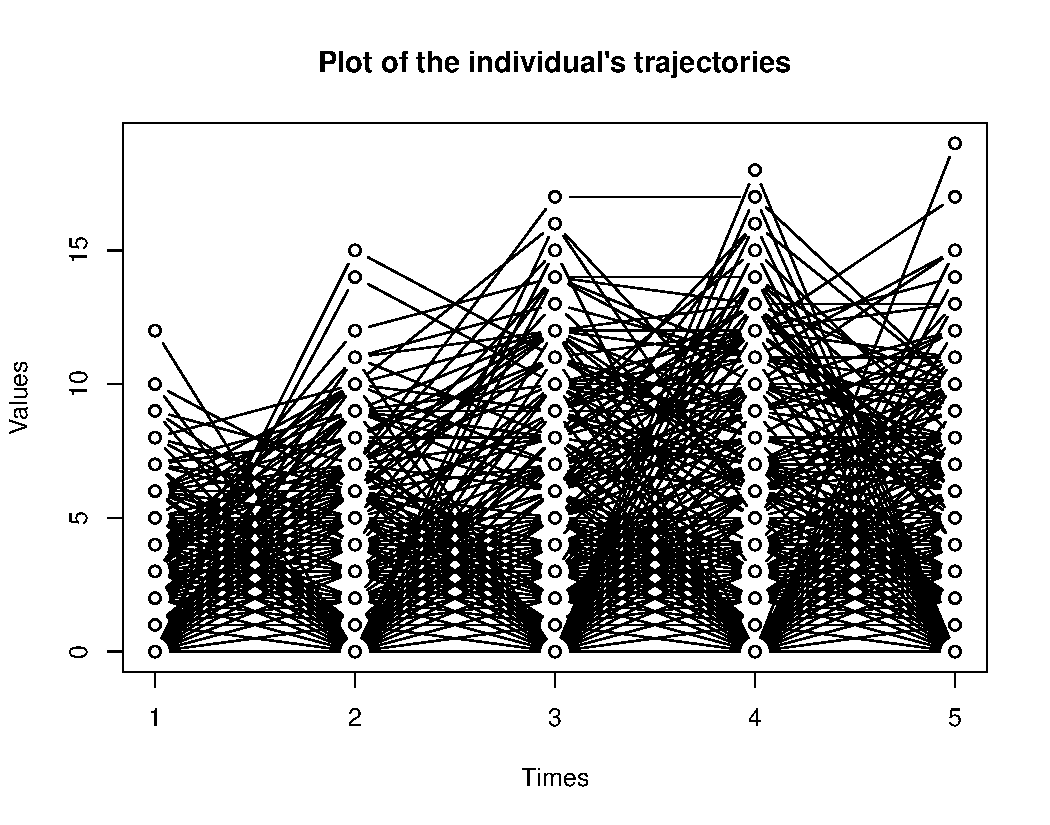
\includegraphics[width=\maxwidth]{figure/unnamed-chunk-49-1} 

\end{knitrout}
We use each method to fit the model. For all method, we specify the number of group of our model, ng=2 and the degree of the polynomial shape of the trajectory for the two state.\\
For the Poisson state we choice a 3 degree polynom and for the zero state a 2 degree polynom.\\
So degree is for $\beta$ a vector $(3,3)$ and for $\nu$ a vector $(2,2)$.\\
We sepcify \verb|hessian=TRUE| to ask the calculus of the hessian matrix.\\
\verb|Itermax | is set to 300 to assure a good approximation of the parameters.\\

For the Likelihood method we call \verb|trajeR| with option \verb|Method ="L"|.
\begin{knitrout}
\definecolor{shadecolor}{rgb}{0.969, 0.969, 0.969}\color{fgcolor}\begin{kframe}
\begin{alltt}
\hlcom{# Likelihood}
\hlstd{paraminit} \hlkwb{=} \hlkwd{c}\hlstd{(}\hlnum{1}\hlstd{,}\hlnum{1}\hlstd{,}
              \hlopt{-}\hlnum{3.066653}\hlstd{,}\hlnum{0}\hlstd{,}\hlnum{0}\hlstd{,}
              \hlopt{-}\hlnum{0.046659}\hlstd{,}\hlnum{0}\hlstd{,}\hlnum{0}\hlstd{,}
              \hlopt{-}\hlnum{3}\hlstd{,}\hlnum{0}\hlstd{,}
              \hlopt{-}\hlnum{3}\hlstd{,}\hlnum{0}\hlstd{)}
\hlstd{solL} \hlkwb{=} \hlkwd{trajeR}\hlstd{(}\hlkwc{Y} \hlstd{= data[,}\hlnum{2}\hlopt{:}\hlnum{6}\hlstd{],} \hlkwc{A} \hlstd{= data[,}\hlnum{7}\hlopt{:}\hlnum{11}\hlstd{],} \hlkwc{ng} \hlstd{=} \hlnum{2}\hlstd{,} \hlkwc{degre}\hlstd{=}\hlkwd{c}\hlstd{(}\hlnum{2}\hlstd{,}\hlnum{2}\hlstd{),} \hlkwc{degre.nu} \hlstd{=} \hlkwd{c}\hlstd{(}\hlnum{1}\hlstd{,}\hlnum{1}\hlstd{),}
              \hlkwc{Model}\hlstd{=}\hlstr{"ZIP"}\hlstd{,} \hlkwc{Method} \hlstd{=} \hlstr{"L"}\hlstd{,} \hlkwc{hessian} \hlstd{=} \hlnum{TRUE}\hlstd{,}
              \hlkwc{paraminit} \hlstd{= paraminit)}
\end{alltt}
\end{kframe}
\end{knitrout}
\begin{knitrout}
\definecolor{shadecolor}{rgb}{0.969, 0.969, 0.969}\color{fgcolor}\begin{kframe}
\begin{alltt}
\hlstd{solL}
\end{alltt}
\begin{verbatim}
## Call TrajeR with 2 groups and a 2,2 degrees of polynomial shape of trajectory.
## Model : Zero Inflated Poisson
## Method : Likelihood 
##  
##   group   Parameter   Estimate   Std. Error   T for H0:   Prob>|T|  
##                                                param.=0             
## --------------------------------------------------------------------
##       1   Intercept    1.04873      0.09415    11.13945          0  
##              Linear    0.61506      0.06423     9.57663          0  
##           Quadratic   -0.07773      0.00998    -7.79183          0  
##                Nu11    0.03161      0.16749     0.18871    0.85034  
##                Nu12   -0.16776      0.05183    -3.23661    0.00123  
##                                                                     
##       2   Intercept    0.90787      0.09589      9.4679          0  
##              Linear    0.01869      0.07032      0.2658    0.79042  
##           Quadratic    0.00619      0.01131     0.54724    0.58426  
##                Nu21   -1.08139      0.16018    -6.75111          0  
##                Nu22    0.00452      0.04689     0.09632    0.92327  
## --------------------------------------------------------------------
##       1         pi1    0.34869      0.04936    13.93138          0  
##       2         pi2    0.65131      0.04936    26.59044          0  
## --------------------------------------------------------------------
## Likelihood : -5162.009
\end{verbatim}
\end{kframe}
\end{knitrout}
For use EM method we write the same syntax but change the variable \verb|Method| to \verb|EM| or \verb|EMIRLS|. In the first case, we find the parameters with quasi newton method and in the second one with Iterative Reweighted Least Square.
\begin{knitrout}
\definecolor{shadecolor}{rgb}{0.969, 0.969, 0.969}\color{fgcolor}\begin{kframe}
\begin{alltt}
\hlcom{# EM}
\hlstd{paraminitEM} \hlkwb{=} \hlkwd{c}\hlstd{(}\hlnum{0.5}\hlstd{,}\hlnum{0.5}\hlstd{,}
                \hlopt{-}\hlnum{3.066653}\hlstd{,}\hlnum{0}\hlstd{,}\hlnum{0}\hlstd{,}
                \hlopt{-}\hlnum{0.046659}\hlstd{,}\hlnum{0}\hlstd{,}\hlnum{0}\hlstd{,}
                \hlopt{-}\hlnum{3}\hlstd{,}\hlnum{0}\hlstd{,}
                \hlopt{-}\hlnum{3}\hlstd{,}\hlnum{0}\hlstd{)}
\hlstd{solEM} \hlkwb{=} \hlkwd{trajeR}\hlstd{(}\hlkwc{Y} \hlstd{= data[,}\hlnum{2}\hlopt{:}\hlnum{6}\hlstd{],} \hlkwc{A} \hlstd{= data[,}\hlnum{7}\hlopt{:}\hlnum{11}\hlstd{],}
               \hlkwc{ng} \hlstd{=} \hlnum{2}\hlstd{,} \hlkwc{degre}\hlstd{=}\hlkwd{c}\hlstd{(}\hlnum{2}\hlstd{,}\hlnum{2}\hlstd{),} \hlkwc{degre.nu} \hlstd{=} \hlkwd{c}\hlstd{(}\hlnum{1}\hlstd{,}\hlnum{1}\hlstd{),}
               \hlkwc{Model}\hlstd{=}\hlstr{"ZIP"}\hlstd{,} \hlkwc{Method} \hlstd{=} \hlstr{"EM"}\hlstd{,} \hlkwc{hessian} \hlstd{=} \hlnum{TRUE}\hlstd{,}
               \hlkwc{paraminit} \hlstd{= paraminitEM)}
\hlstd{paraminitEMIRLS} \hlkwb{=} \hlkwd{c}\hlstd{(}\hlnum{0.5}\hlstd{,}\hlnum{0.5}\hlstd{,}
                    \hlopt{-}\hlnum{1.540445}\hlstd{,}\hlnum{0}\hlstd{,}\hlnum{0}\hlstd{,}
                    \hlnum{0}\hlstd{,}\hlnum{0}\hlstd{,}\hlnum{0}\hlstd{,}
                    \hlopt{-}\hlnum{3}\hlstd{,}\hlnum{0}\hlstd{,}
                    \hlopt{-}\hlnum{3}\hlstd{,}\hlnum{0}\hlstd{)}
\hlstd{solEMIRLS} \hlkwb{=} \hlkwd{trajeR}\hlstd{(}\hlkwc{Y} \hlstd{= data[,}\hlnum{2}\hlopt{:}\hlnum{6}\hlstd{],} \hlkwc{A} \hlstd{= data[,}\hlnum{7}\hlopt{:}\hlnum{11}\hlstd{],}
                   \hlkwc{ng} \hlstd{=} \hlnum{2}\hlstd{,} \hlkwc{degre}\hlstd{=}\hlkwd{c}\hlstd{(}\hlnum{2}\hlstd{,}\hlnum{2}\hlstd{),} \hlkwc{degre.nu} \hlstd{=} \hlkwd{c}\hlstd{(}\hlnum{1}\hlstd{,}\hlnum{1}\hlstd{),}
                   \hlkwc{Model}\hlstd{=}\hlstr{"ZIP"}\hlstd{,} \hlkwc{Method} \hlstd{=} \hlstr{"EMIRLS"}\hlstd{,} \hlkwc{hessian} \hlstd{=} \hlnum{TRUE}\hlstd{,}
                   \hlkwc{paraminit} \hlstd{= paraminitEM)}
\end{alltt}
\end{kframe}
\end{knitrout}


\begin{table}[H]
\centering
\begin{tabular}{rrrrrr}
\toprule
\multicolumn{2}{c}{SolL} & \multicolumn{2}{c}{SolEM} & \multicolumn{2}{c}{SolEMIRLS} \\
\cmidrule(l{3pt}r{3pt}){1-2} \cmidrule(l{3pt}r{3pt}){3-4} \cmidrule(l{3pt}r{3pt}){5-6}
parameters & sd & parameters & sd & parameters & sd\\
\midrule
\addlinespace[0.3em]
\multicolumn{6}{l}{\textbf{Beta 1}}\\
\hspace{1em}1.04873 & 0.09415 & 0.90771 & 0.07864 & 0.90782 & 0.07864\\
\hspace{1em}0.61506 & 0.06423 & 0.01879 & 0.05853 & 0.01872 & 0.05853\\
\hspace{1em}-0.07773 & 0.00998 & 0.00617 & 0.00947 & 0.00618 & 0.00947\\
\addlinespace[0.3em]
\multicolumn{6}{l}{\textbf{Beta 2}}\\
\hspace{1em}0.90787 & 0.09589 & 1.04852 & 0.07780 & 1.04873 & 0.07779\\
\hspace{1em}0.01869 & 0.07032 & 0.61510 & 0.05281 & 0.61507 & 0.05281\\
\hspace{1em}0.00619 & 0.01131 & -0.07773 & 0.00818 & -0.07773 & 0.00818\\
\addlinespace[0.3em]
\multicolumn{6}{l}{\textbf{Nu 1}}\\
\hspace{1em}0.03161 & 0.16749 & -1.08155 & 0.16533 & -1.08146 & 0.16533\\
\hspace{1em}-0.16776 & 0.05183 & 0.00456 & 0.04874 & 0.00454 & 0.04874\\
\addlinespace[0.3em]
\multicolumn{6}{l}{\textbf{Nu 2}}\\
\hspace{1em}-1.08139 & 0.16018 & 0.03158 & 0.18598 & 0.03162 & 0.18598\\
\hspace{1em}0.00452 & 0.04689 & -0.16775 & 0.05729 & -0.16776 & 0.05729\\
\addlinespace[0.3em]
\multicolumn{6}{l}{\textbf{Pi}}\\
\hspace{1em}0.34869 & 0.04936 & 0.65131 & 0.02388 & 0.65132 & 0.02388\\
\hspace{1em}0.65131 & 0.04936 & 0.34869 & 0.02388 & 0.34868 & 0.02388\\
\bottomrule
\end{tabular}
\end{table}



\subsection{Plot}
We plot only the trajectory on a graph. We have just to use the native plot function. It use the class of the object to draw the polynomial shape. The values in abscissa are the first row of the time variable.

\begin{knitrout}
\definecolor{shadecolor}{rgb}{0.969, 0.969, 0.969}\color{fgcolor}\begin{kframe}
\begin{alltt}
\hlkwd{plot}\hlstd{(solL)}
\end{alltt}
\end{kframe}
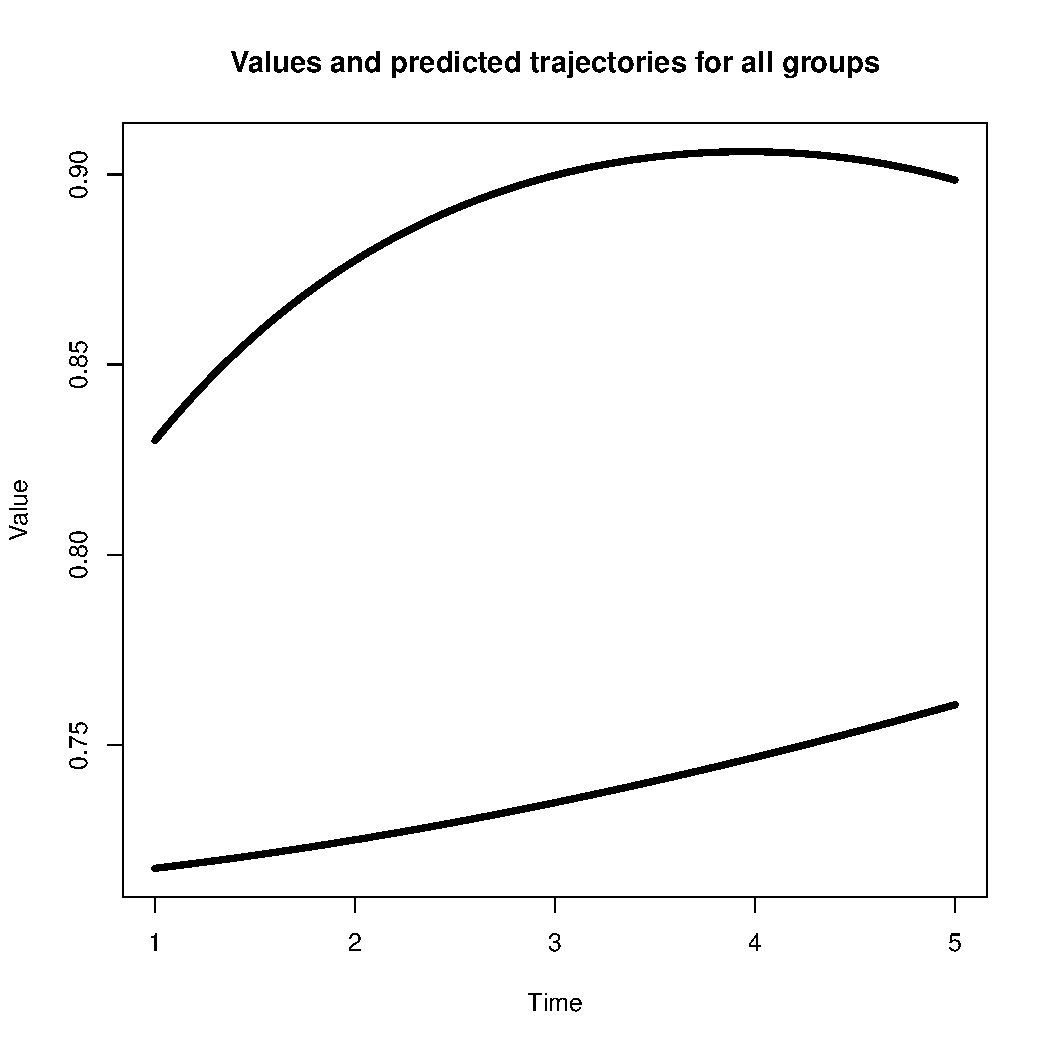
\includegraphics[width=\maxwidth]{figure/unnamed-chunk-55-1} 

\end{knitrout}
We can add longitudinal data to this graph. If we want this on the plot we have to specify \verb|Y| and \verb|A| in the function \verb|plot()|. For more visibility, we have enlarge the 0 and 1 value on the graph and plot the data with a little and random shift, control by the index \verb|dec| in the function plot.\\
By default colors are gray scale, but we can specify colors we want.

\begin{knitrout}
\definecolor{shadecolor}{rgb}{0.969, 0.969, 0.969}\color{fgcolor}\begin{kframe}
\begin{alltt}
\hlcom{# colour's defintion}
\hlstd{trans} \hlkwb{=} \hlstr{"70"}
\hlstd{col1} \hlkwb{=} \hlstr{"#034569"}
\hlstd{col1.1} \hlkwb{=} \hlkwd{paste0}\hlstd{(}\hlstr{"#64AAD0"}\hlstd{, trans)}
\hlstd{col2} \hlkwb{=} \hlstr{"#750062"}
\hlstd{col2.1} \hlkwb{=} \hlkwd{paste0}\hlstd{(}\hlstr{"#D962C7"}\hlstd{, trans)}
\hlstd{cols1} \hlkwb{=} \hlkwd{c}\hlstd{(col1.1, col2.1)}
\hlstd{cols2} \hlkwb{=} \hlkwd{c}\hlstd{(col1, col2)}
\hlstd{vcol} \hlkwb{=} \hlkwd{c}\hlstd{(cols1, cols2)}

\hlkwd{plot}\hlstd{(solEM,} \hlkwc{Y} \hlstd{= dataZIP[,}\hlnum{2}\hlopt{:}\hlnum{6}\hlstd{],} \hlkwc{A} \hlstd{= dataZIP[,}\hlnum{7}\hlopt{:}\hlnum{11}\hlstd{],} \hlkwc{dec} \hlstd{=} \hlnum{5}\hlstd{,} \hlkwc{col} \hlstd{= vcol)}
\end{alltt}
\end{kframe}
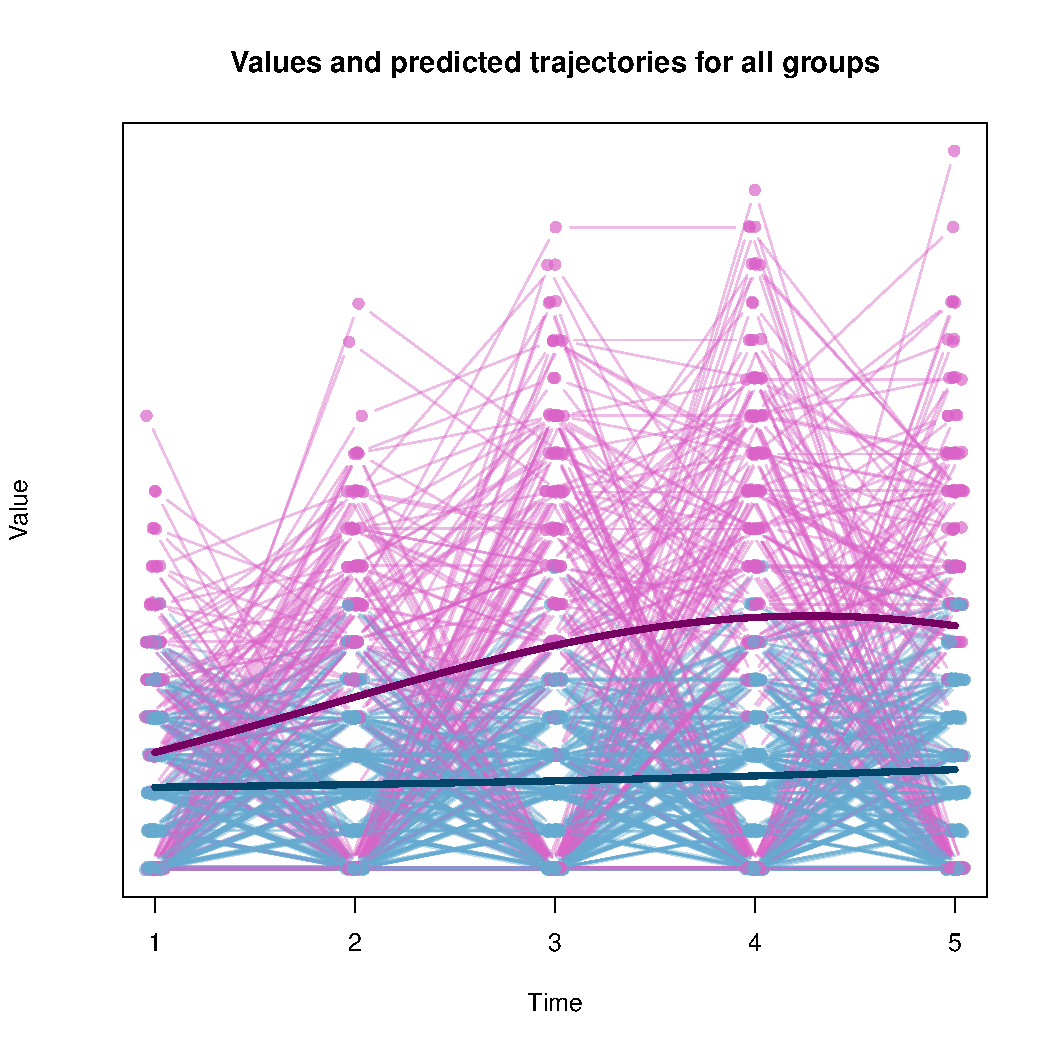
\includegraphics[width=\maxwidth]{figure/unnamed-chunk-56-1} 

\end{knitrout}

\subsection{Adding covariate}
In the same way that in the section below we can add covariate in the calculus of the parameters. \\

If we add risk variable we use option \verb|Risk =|.
\begin{knitrout}
\definecolor{shadecolor}{rgb}{0.969, 0.969, 0.969}\color{fgcolor}\begin{kframe}
\begin{alltt}
\hlstd{solLRisk} \hlkwb{=} \hlkwd{trajeR}\hlstd{(}\hlkwc{Y} \hlstd{= data[,}\hlnum{2}\hlopt{:}\hlnum{6}\hlstd{],} \hlkwc{A} \hlstd{= data[,}\hlnum{7}\hlopt{:}\hlnum{11}\hlstd{],} \hlkwc{Risk} \hlstd{= data[,}\hlnum{12}\hlstd{],}
                  \hlkwc{ng} \hlstd{=} \hlnum{2}\hlstd{,} \hlkwc{degre}\hlstd{=}\hlkwd{c}\hlstd{(}\hlnum{2}\hlstd{,}\hlnum{2}\hlstd{),} \hlkwc{degre.nu} \hlstd{=} \hlkwd{c}\hlstd{(}\hlnum{1}\hlstd{,}\hlnum{1}\hlstd{),}
                  \hlkwc{Model}\hlstd{=}\hlstr{"ZIP"}\hlstd{,} \hlkwc{Method} \hlstd{=} \hlstr{"L"}\hlstd{,} \hlkwc{hessian} \hlstd{=} \hlnum{TRUE}\hlstd{,}
                  \hlkwc{paraminit} \hlstd{= paraminit)}
\end{alltt}
\end{kframe}
\end{knitrout}
\begin{knitrout}
\definecolor{shadecolor}{rgb}{0.969, 0.969, 0.969}\color{fgcolor}\begin{kframe}
\begin{alltt}
\hlstd{solLRisk}
\end{alltt}
\begin{verbatim}
## Call TrajeR with 2 groups and a 2,2 degrees of polynomial shape of trajectory.
## Model : Zero Inflated Poisson
## Method : Likelihood 
##  
##   group   Parameter   Estimate   Std. Error   T for H0:   Prob>|T|  
##                                                param.=0             
## --------------------------------------------------------------------
##       1   Intercept    1.04843      0.09888    10.60333          0  
##              Linear    0.61501      0.16707     3.68117    0.00024  
##           Quadratic   -0.07772      0.09411     -0.8258      0.409  
##                Nu11    0.03215       0.0703     0.45738    0.64744  
##                Nu12   -0.16784      0.01131   -14.84504          0  
##                                                                     
##       2   Intercept    0.90742       0.0642    14.13335          0  
##              Linear    0.01907      0.00997     1.91259    0.05592  
##           Quadratic     0.0061      0.09582     0.06363    0.94927  
##                Nu21   -1.08237       0.1674    -6.46565          0  
##                Nu22    0.00462      0.05179      0.0892    0.92893  
## --------------------------------------------------------------------
##       1    Baseline          0      0.16034     3.69222    0.00023  
##                                                                     
##       2   Intercept    0.81597      0.09888    14.23977          0  
##                   X   -0.37654      0.16707    -1.12689     0.2599  
## --------------------------------------------------------------------
## Likelihood : -5161.373
\end{verbatim}
\end{kframe}
\end{knitrout}
We can use all method too.
\begin{knitrout}
\definecolor{shadecolor}{rgb}{0.969, 0.969, 0.969}\color{fgcolor}\begin{kframe}
\begin{alltt}
\hlstd{solEMRisk} \hlkwb{=} \hlkwd{trajeR}\hlstd{(}\hlkwc{Y} \hlstd{= data[,}\hlnum{2}\hlopt{:}\hlnum{6}\hlstd{],} \hlkwc{A} \hlstd{= data[,}\hlnum{7}\hlopt{:}\hlnum{11}\hlstd{],} \hlkwc{Risk} \hlstd{= data[,}\hlnum{12}\hlstd{],}
                   \hlkwc{ng} \hlstd{=} \hlnum{2}\hlstd{,} \hlkwc{degre}\hlstd{=}\hlkwd{c}\hlstd{(}\hlnum{2}\hlstd{,}\hlnum{2}\hlstd{),} \hlkwc{degre.nu} \hlstd{=} \hlkwd{c}\hlstd{(}\hlnum{1}\hlstd{,}\hlnum{1}\hlstd{),}
                   \hlkwc{Model}\hlstd{=}\hlstr{"ZIP"}\hlstd{,} \hlkwc{Method} \hlstd{=} \hlstr{"EM"}\hlstd{,} \hlkwc{hessian} \hlstd{=} \hlnum{TRUE}\hlstd{,}
                   \hlkwc{paraminit} \hlstd{= paraminit)}
\hlstd{solEMIRLSRisk} \hlkwb{=} \hlkwd{trajeR}\hlstd{(}\hlkwc{Y} \hlstd{= data[,}\hlnum{2}\hlopt{:}\hlnum{6}\hlstd{],} \hlkwc{A} \hlstd{= data[,}\hlnum{7}\hlopt{:}\hlnum{11}\hlstd{],} \hlkwc{Risk} \hlstd{= data[,}\hlnum{12}\hlstd{],}
                       \hlkwc{ng} \hlstd{=} \hlnum{2}\hlstd{,} \hlkwc{degre}\hlstd{=}\hlkwd{c}\hlstd{(}\hlnum{2}\hlstd{,}\hlnum{2}\hlstd{),} \hlkwc{degre.nu} \hlstd{=} \hlkwd{c}\hlstd{(}\hlnum{1}\hlstd{,}\hlnum{1}\hlstd{),}
                       \hlkwc{Model}\hlstd{=}\hlstr{"ZIP"}\hlstd{,} \hlkwc{Method} \hlstd{=} \hlstr{"EMIRLS"}\hlstd{,} \hlkwc{hessian} \hlstd{=} \hlnum{FALSE}\hlstd{,}
                       \hlkwc{paraminit} \hlstd{= paraminit)}
\end{alltt}
\end{kframe}
\end{knitrout}
We have


\begin{table}[H]
\centering
\begin{tabular}{rrrrrr}
\toprule
\multicolumn{2}{c}{SolLRisk} & \multicolumn{2}{c}{SolEMRisk} & \multicolumn{2}{c}{SolEMIRLSRisk} \\
\cmidrule(l{3pt}r{3pt}){1-2} \cmidrule(l{3pt}r{3pt}){3-4} \cmidrule(l{3pt}r{3pt}){5-6}
parameters & sd & parameters & sd & parameters & sd\\
\midrule
\addlinespace[0.3em]
\multicolumn{6}{l}{\textbf{Beta 1}}\\
\hspace{1em}1.04843 & 0.09888 & 1.05048 & 0.0744032 & 1.05107 & 0.07440\\
\hspace{1em}0.61501 & 0.16707 & 0.61630 & 0.0499435 & 0.61579 & 0.04994\\
\hspace{1em}-0.07772 & 0.09411 & -0.07795 & 0.0077179 & -0.07786 & 0.00772\\
\addlinespace[0.3em]
\multicolumn{6}{l}{\textbf{Beta 2}}\\
\hspace{1em}0.90742 & 0.06420 & 0.91182 & 0.0784344 & 0.91173 & 0.07844\\
\hspace{1em}0.01907 & 0.00997 & 0.01766 & 0.0584119 & 0.01772 & 0.05841\\
\hspace{1em}0.00610 & 0.09582 & 0.00641 & 0.0094507 & 0.00640 & 0.00945\\
\addlinespace[0.3em]
\multicolumn{6}{l}{\textbf{Nu 1}}\\
\hspace{1em}0.03215 & 0.07030 & 0.03362 & 0.1852634 & 0.03362 & 0.18526\\
\hspace{1em}-0.16784 & 0.01131 & -0.17080 & 0.0569155 & -0.17079 & 0.05692\\
\addlinespace[0.3em]
\multicolumn{6}{l}{\textbf{Nu 2}}\\
\hspace{1em}-1.08237 & 0.16740 & -1.07298 & 0.1638207 & -1.07300 & 0.16383\\
\hspace{1em}0.00462 & 0.05179 & 0.00502 & 0.0482664 & 0.00502 & 0.04827\\
\addlinespace[0.3em]
\multicolumn{6}{l}{\textbf{Theta}}\\
\hspace{1em}0.00000 & 0.16034 & 0.00000 & 0.0000000 & 0.00000 & 0.00000\\
\hspace{1em}0.00000 & 0.04693 & 0.00000 & 0.0000000 & 0.00000 & 0.00000\\
\hspace{1em}-0.81598 & 0.09888 & 0.81719 & 0.1979696 & -0.81717 & 0.19797\\
\hspace{1em}0.37654 & 0.16707 & -0.34178 & 0.3347726 & 0.34180 & 0.33477\\
\bottomrule
\end{tabular}
\end{table}



\subsection{Adding time depdendent covariate}
If we add time dependent covariate we use option \verb|TCOV|.
\begin{knitrout}
\definecolor{shadecolor}{rgb}{0.969, 0.969, 0.969}\color{fgcolor}\begin{kframe}
\begin{alltt}
\hlstd{paraminit}\hlkwb{=}\hlkwd{c}\hlstd{(}\hlnum{1}\hlstd{,}\hlnum{1}\hlstd{,}
            \hlopt{-}\hlnum{0.738409}\hlstd{,}\hlnum{0}\hlstd{,}\hlnum{0}\hlstd{,}
            \hlnum{0.489316}\hlstd{,}\hlnum{0}\hlstd{,}\hlnum{0}\hlstd{,}
            \hlopt{-}\hlnum{3}\hlstd{,} \hlnum{0}\hlstd{,}
            \hlopt{-}\hlnum{3}\hlstd{,} \hlnum{0}\hlstd{,}
            \hlnum{0}\hlstd{,} \hlnum{0}\hlstd{)}
\hlstd{solLTCOV} \hlkwb{=} \hlkwd{trajeR}\hlstd{(}\hlkwc{Y} \hlstd{= data[,}\hlnum{2}\hlopt{:}\hlnum{6}\hlstd{],} \hlkwc{A} \hlstd{= data[,}\hlnum{7}\hlopt{:}\hlnum{11}\hlstd{],} \hlkwc{TCOV} \hlstd{= data[,}\hlnum{13}\hlopt{:}\hlnum{17}\hlstd{],}
                  \hlkwc{ng} \hlstd{=} \hlnum{2}\hlstd{,} \hlkwc{degre}\hlstd{=}\hlkwd{c}\hlstd{(}\hlnum{2}\hlstd{,}\hlnum{2}\hlstd{),} \hlkwc{degre.nu} \hlstd{=} \hlkwd{c}\hlstd{(}\hlnum{1}\hlstd{,}\hlnum{1}\hlstd{),}
                  \hlkwc{Model}\hlstd{=}\hlstr{"ZIP"}\hlstd{,} \hlkwc{Method} \hlstd{=} \hlstr{"L"}\hlstd{,} \hlkwc{hessian} \hlstd{=} \hlnum{TRUE}\hlstd{,}
                  \hlkwc{paraminit} \hlstd{= paraminit)}
\end{alltt}
\end{kframe}
\end{knitrout}
\begin{knitrout}
\definecolor{shadecolor}{rgb}{0.969, 0.969, 0.969}\color{fgcolor}\begin{kframe}
\begin{alltt}
\hlstd{solLTCOV}
\end{alltt}
\begin{verbatim}
## Call TrajeR with 2 groups and a 2,2 degrees of polynomial shape of trajectory.
## Model : Zero Inflated Poisson
## Method : Likelihood 
##  
##   group   Parameter   Estimate   Std. Error   T for H0:   Prob>|T|  
##                                                param.=0             
## --------------------------------------------------------------------
##       1   Intercept    0.88075           NA          NA         NA  
##              Linear    0.01537           NA          NA         NA  
##           Quadratic    0.00677           NA          NA         NA  
##                Nu11   -1.07075           NA          NA         NA  
##                Nu12    0.00233           NA          NA         NA  
##               TCOV1    0.06375           NA          NA         NA  
##                                                                     
##       2   Intercept    1.04297           NA          NA         NA  
##              Linear    0.61471           NA          NA         NA  
##           Quadratic   -0.07767           NA          NA         NA  
##                Nu21    0.02795           NA          NA         NA  
##                Nu22   -0.16711           NA          NA         NA  
##               TCOV1    0.01295           NA          NA         NA  
## --------------------------------------------------------------------
##       1         pi1    0.65197           NA          NA         NA  
##       2         pi2    0.34803           NA          NA         NA  
## --------------------------------------------------------------------
## Likelihood : -5160.531
\end{verbatim}
\end{kframe}
\end{knitrout}
We can use all method too.
\begin{knitrout}
\definecolor{shadecolor}{rgb}{0.969, 0.969, 0.969}\color{fgcolor}\begin{kframe}
\begin{alltt}
\hlstd{solEMTCOV} \hlkwb{=} \hlkwd{trajeR}\hlstd{(}\hlkwc{Y} \hlstd{= data[,}\hlnum{2}\hlopt{:}\hlnum{6}\hlstd{],} \hlkwc{A} \hlstd{= data[,}\hlnum{7}\hlopt{:}\hlnum{11}\hlstd{],} \hlkwc{TCOV} \hlstd{= data[,}\hlnum{13}\hlopt{:}\hlnum{17}\hlstd{],}
                   \hlkwc{ng} \hlstd{=} \hlnum{2}\hlstd{,} \hlkwc{degre}\hlstd{=}\hlkwd{c}\hlstd{(}\hlnum{2}\hlstd{,}\hlnum{2}\hlstd{),} \hlkwc{degre.nu} \hlstd{=} \hlkwd{c}\hlstd{(}\hlnum{1}\hlstd{,}\hlnum{1}\hlstd{),}
                   \hlkwc{Model}\hlstd{=}\hlstr{"ZIP"}\hlstd{,} \hlkwc{Method} \hlstd{=} \hlstr{"EM"}\hlstd{,} \hlkwc{hessian} \hlstd{=} \hlnum{TRUE}\hlstd{,}
                   \hlkwc{paraminit} \hlstd{= paraminitEM)}
\hlstd{solEMIRLSTCOV} \hlkwb{=} \hlkwd{trajeR}\hlstd{(}\hlkwc{Y} \hlstd{= data[,}\hlnum{2}\hlopt{:}\hlnum{6}\hlstd{],} \hlkwc{A} \hlstd{= data[,}\hlnum{7}\hlopt{:}\hlnum{11}\hlstd{],} \hlkwc{TCOV} \hlstd{= data[,}\hlnum{13}\hlopt{:}\hlnum{17}\hlstd{],}
                       \hlkwc{ng} \hlstd{=} \hlnum{2}\hlstd{,} \hlkwc{degre}\hlstd{=}\hlkwd{c}\hlstd{(}\hlnum{2}\hlstd{,}\hlnum{2}\hlstd{),} \hlkwc{degre.nu} \hlstd{=} \hlkwd{c}\hlstd{(}\hlnum{1}\hlstd{,}\hlnum{1}\hlstd{),}
                       \hlkwc{Model}\hlstd{=}\hlstr{"ZIP"}\hlstd{,} \hlkwc{Method} \hlstd{=} \hlstr{"EMIRLS"}\hlstd{,} \hlkwc{hessian} \hlstd{=} \hlnum{TRUE}\hlstd{,}
                       \hlkwc{paraminit} \hlstd{= paraminitEM)}
\end{alltt}
\end{kframe}
\end{knitrout}
We have

\begin{table}[H]
\centering
\begin{tabular}{rrr}
\toprule
SolLTCOV & SolEMTCOV & SoEMIRLSTCOV\\
\midrule
\addlinespace[0.3em]
\multicolumn{3}{l}{\textbf{Beta 1}}\\
\hspace{1em}0.88075 & 0.87432 & 0.87514\\
\hspace{1em}0.01537 & 0.01821 & 0.01789\\
\hspace{1em}0.00677 & 0.00642 & 0.00646\\
\addlinespace[0.3em]
\multicolumn{3}{l}{\textbf{Beta 2}}\\
\hspace{1em}1.04297 & 1.04159 & 1.04243\\
\hspace{1em}0.61471 & 0.61510 & 0.61456\\
\hspace{1em}-0.07767 & -0.07772 & -0.07764\\
\addlinespace[0.3em]
\multicolumn{3}{l}{\textbf{Nu 1}}\\
\hspace{1em}-1.07075 & -1.09978 & -1.09925\\
\hspace{1em}0.00233 & 0.00542 & 0.00531\\
\addlinespace[0.3em]
\multicolumn{3}{l}{\textbf{Nu 2}}\\
\hspace{1em}0.02795 & 0.02772 & 0.02781\\
\hspace{1em}-0.16711 & -0.16645 & -0.16649\\
\addlinespace[0.3em]
\multicolumn{3}{l}{\textbf{TCOV}}\\
\hspace{1em}0.06375 & 0.05647 & 0.05631\\
\hspace{1em}0.01295 & 0.01307 & 0.01303\\
\addlinespace[0.3em]
\multicolumn{3}{l}{\textbf{Pi}}\\
\hspace{1em}0.65197 & 0.65108 & 0.65109\\
\hspace{1em}0.34803 & 0.34892 & 0.34891\\
\bottomrule
\end{tabular}
\end{table}


We can add the effect of other time covariate.

\begin{knitrout}
\definecolor{shadecolor}{rgb}{0.969, 0.969, 0.969}\color{fgcolor}
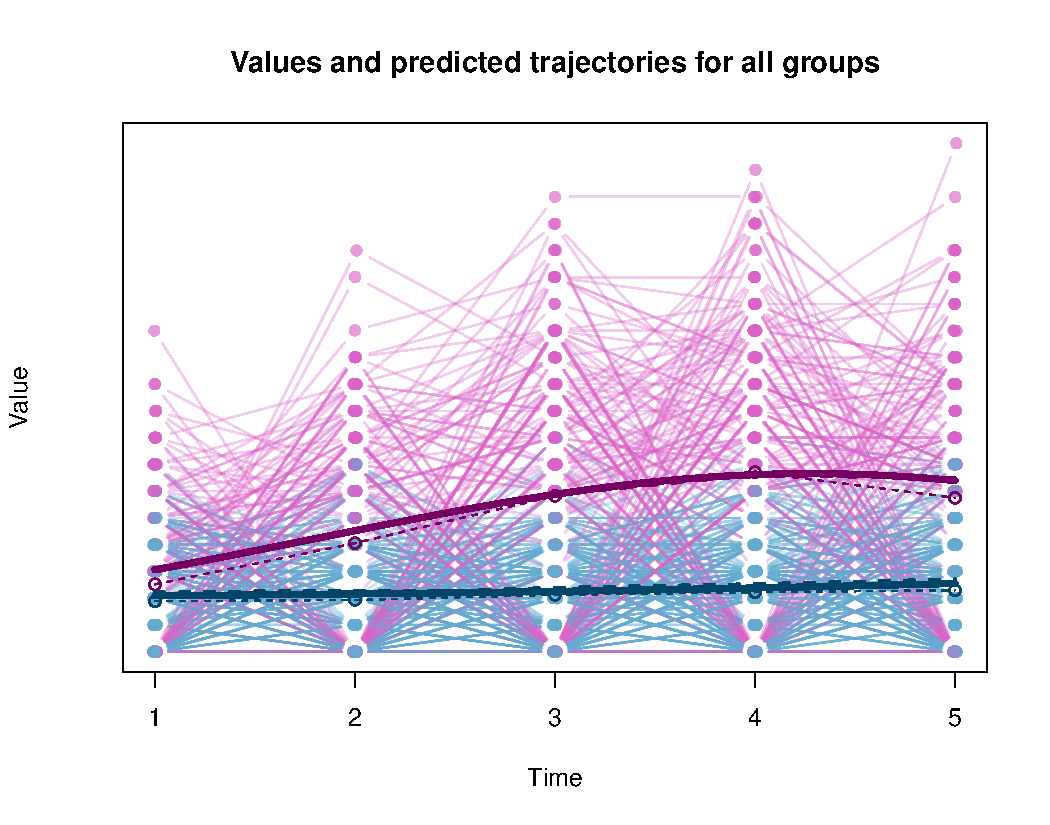
\includegraphics[width=\maxwidth]{figure/unnamed-chunk-67-1} 

\end{knitrout}

\section{Non Linear model}

We suppose that the variable $Y_{it}$ is defined by
\begin{equation}
y_{it} = f(a_{it}; \beta_k)+\epsilon_{it}
\end{equation}
where $\epsilon_{it}\sim \mathcal{N}\left(0;\ \sigma_k\right)$.\\


In this case, the function $f_k$ is not linear in the parameters $\beta_k$ and

\begin{equation}
	E(Y_{it}=y_{it}|W_i=w_i,C_i=k)=  f(a_{it}; \beta_k)
\end{equation}

We note $\phi$ the density function of a normal distribution with mean 0 and standard deviation 1 and $\Phi$ its  cumulative distribution function, if we fit a group $k$ we can write


\begin{align}
P(Y_{it}=y_{it}|W_i=w_i,C_i=k)=
\dfrac{1}{\sigma_k}\phi\left(\dfrac{y_{it}- f(a_{it}; \beta_k)}{\sigma_k}\right)
\end{align}

\subsection{Parameters}

\textbf{Example}\\
We use artificial data contained in the library. This are 500 longitudinal data generate by the parameters above :
\begin{itemize}
	\item 4 groups ;
	\item probability is $\pi_1=0.2$, $\pi_2=0.3$, $\pi_3=0.14$ and $\pi_4=0.36$ ;
	\item period is 11 ;
	\item $\sigma_1=0.45$, $\sigma_2=0.65$, $\sigma_3=0.35$ and $\sigma_4=0.4$.
	\item the link\footnote{it is the Michaelis–Menten equation.}  function between individuals and paramaters is
	\[f(t; \beta_k) =\frac{\beta_{k1}t}{\beta_{k2} + t}\]

	\item the parameters\footnote{the informed reader will have recognized, in order, \textit{Glutamate dehydrogenase} in NAD\textsuperscript{+}, \textit{Pyruvate carboxylaste} in ATP, \textit{Threonine deaminase} in Threonine and \textit{Hexokinase} in Fructose.} are $\beta_1=(3.6,0.025)$, $\beta_2=(2.9,0.06)$, $\beta_3=(3.4,5)$ and $\beta_4=(3.4,1.5)$.
\end{itemize}

The data contains the time variable dependent $Y_i$ in \verb|data[,2:12]|, the time variable in \verb|data[,13:23]|.
\begin{itemize}
	\item \verb|data[,2:12]| is a matrix withe real.
	\item \verb|data[,13:23]| is a matrix with time 0 to 10.
\end{itemize}



\begin{knitrout}
\definecolor{shadecolor}{rgb}{0.969, 0.969, 0.969}\color{fgcolor}
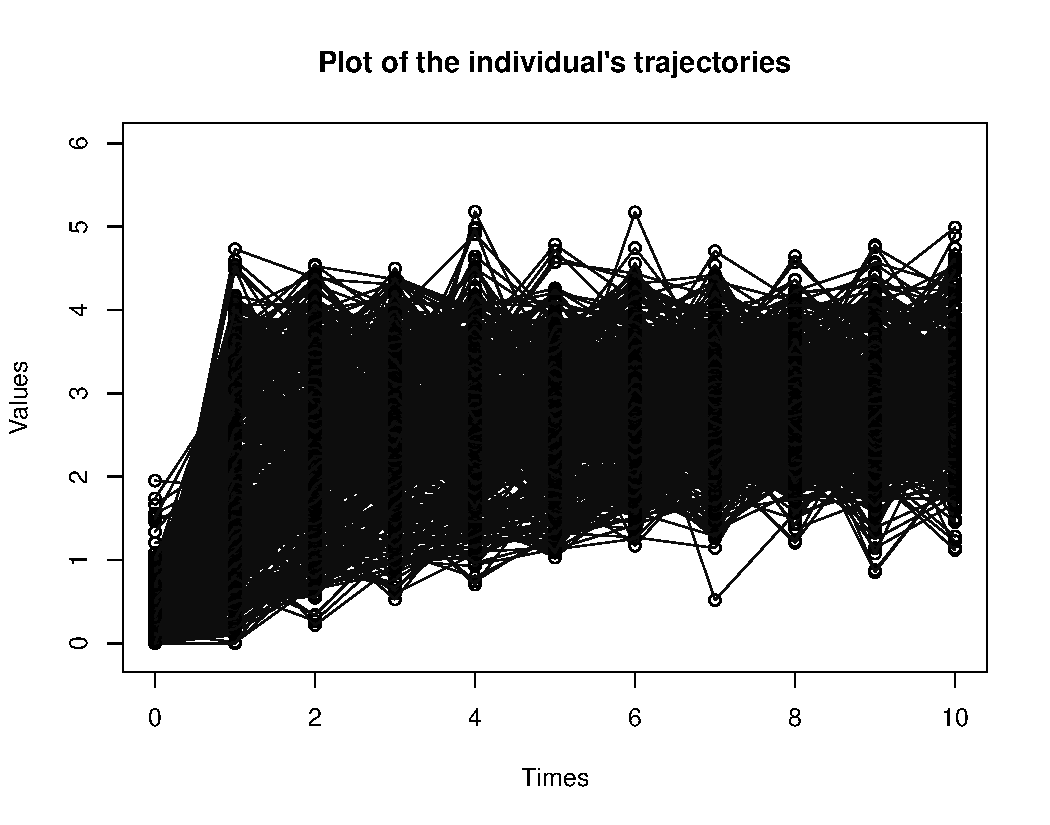
\includegraphics[width=\maxwidth]{figure/unnamed-chunk-69-1} 

\end{knitrout}
We use the non linear method to fit the model. We specify the number of group \verb|ng| to 4 and the number of parameters \verb|nbvar| to 2.
We sepcify too \verb|hessian=TRUE| to ask the calculus of the hessian matrix.\\
\verb|Itermax | is set to 300 to assure a good approximation of the parameters.\\

We call \verb|trajeR| with option \verb|Method ="EM"| and \verb|Model="NL"|. By analysing the graph above, we fit initial parmaters as
\begin{knitrout}
\definecolor{shadecolor}{rgb}{0.969, 0.969, 0.969}\color{fgcolor}\begin{kframe}
\begin{alltt}
\hlstd{paraminit}\hlkwb{=}\hlkwd{c}\hlstd{(}\hlnum{0.25}\hlstd{,}\hlnum{0.25}\hlstd{,}\hlnum{0.25}\hlstd{,}\hlnum{0.25}\hlstd{,}\hlnum{2}\hlstd{,}\hlnum{0.1}\hlstd{,}\hlnum{2.4}\hlstd{,}\hlnum{0.1}\hlstd{,}\hlnum{2.8}\hlstd{,}\hlnum{0.1}\hlstd{,}\hlnum{3}\hlstd{,}\hlnum{0.1}\hlstd{,}\hlnum{0.2}\hlstd{,}\hlnum{0.2}\hlstd{,}\hlnum{0.2}\hlstd{,}\hlnum{0.2}\hlstd{)}
\end{alltt}
\end{kframe}
\end{knitrout}
Then we have to define the link function and its differential.
\begin{knitrout}
\definecolor{shadecolor}{rgb}{0.969, 0.969, 0.969}\color{fgcolor}\begin{kframe}
\begin{alltt}
\hlcom{#defintion of the function}
\hlstd{fct} \hlkwb{<-} \hlkwa{function}\hlstd{(}\hlkwc{t}\hlstd{,} \hlkwc{betak}\hlstd{,} \hlkwc{TCOV}\hlstd{)\{}
  \hlkwd{return}\hlstd{(}
    \hlstd{(betak[}\hlnum{1}\hlstd{]}\hlopt{*}\hlstd{t)}\hlopt{/}\hlstd{(betak[}\hlnum{2}\hlstd{]}\hlopt{+}\hlstd{t)}
  \hlstd{)}
\hlstd{\}}
\hlcom{#defintion of the differential}
\hlstd{diffct} \hlkwb{<-} \hlkwa{function}\hlstd{(}\hlkwc{t}\hlstd{,} \hlkwc{betak}\hlstd{,} \hlkwc{TCOV}\hlstd{)\{}
  \hlkwd{return}\hlstd{(}\hlkwd{c}\hlstd{(}
    \hlstd{t}\hlopt{/}\hlstd{(betak[}\hlnum{2}\hlstd{]}\hlopt{+}\hlstd{t),}
    \hlopt{-}\hlstd{(betak[}\hlnum{1}\hlstd{]}\hlopt{*}\hlstd{t)}\hlopt{/}\hlstd{(betak[}\hlnum{2}\hlstd{]}\hlopt{+}\hlstd{t)}\hlopt{**}\hlnum{2}
  \hlstd{))}
\hlstd{\}}
\end{alltt}
\end{kframe}
\end{knitrout}
We use the \verb|trajeR| function with the parameters above
\begin{knitrout}
\definecolor{shadecolor}{rgb}{0.969, 0.969, 0.969}\color{fgcolor}\begin{kframe}
\begin{alltt}
\hlstd{solEM} \hlkwb{=} \hlkwd{trajeR}\hlstd{(}\hlkwc{Y} \hlstd{= data[,}\hlnum{2}\hlopt{:}\hlnum{12}\hlstd{],} \hlkwc{A} \hlstd{= data[,}\hlnum{13}\hlopt{:}\hlnum{23}\hlstd{],}
               \hlkwc{ng} \hlstd{=} \hlnum{4}\hlstd{,} \hlkwc{nbvar} \hlstd{=} \hlnum{2}\hlstd{,}
               \hlkwc{Method} \hlstd{=} \hlstr{"EM"}\hlstd{,} \hlkwc{Model} \hlstd{=} \hlstr{"NL"}\hlstd{,} \hlkwc{hessian} \hlstd{=} \hlnum{TRUE}\hlstd{,}
               \hlkwc{fct} \hlstd{= fct,} \hlkwc{diffct} \hlstd{= diffct,} \hlkwc{paraminit} \hlstd{= paraminit)}
\end{alltt}
\end{kframe}
\end{knitrout}
\begin{knitrout}
\definecolor{shadecolor}{rgb}{0.969, 0.969, 0.969}\color{fgcolor}\begin{kframe}
\begin{alltt}
\hlstd{solEM}
\end{alltt}
\begin{verbatim}
## Call TrajeR with 4 groups and a 1,1,1,1 degrees of polynomial shape of trajectory.
## Model : Non Linear
## Method : Expectation-maximization 
##  
##   group   Parameter   Estimate   Std. Error   T for H0:   Prob>|T|  
##                                                param.=0             
## --------------------------------------------------------------------
##       1   Intercept    3.30547      0.11174     29.5806          0  
##              Linear    4.72453      0.36521    12.93659          0  
##                                                                     
##       2   Intercept    3.40216      0.04909    69.30994          0  
##              Linear    1.52195      0.09214    16.51695          0  
##                                                                     
##       3   Intercept    2.88488      0.02227   129.54035          0  
##              Linear    0.04596      0.02132     2.15543    0.03117  
##                                                                     
##       4   Intercept    3.65116      0.02245   162.66989          0  
##              Linear    0.03562      0.01594     2.23507    0.02545  
## --------------------------------------------------------------------
##       1      sigma1    0.34668      0.00842     41.1552          0  
##       2      sigma2    0.39863      0.00725    55.01187          0  
##       3      sigma3    0.64933      0.01148    56.54777          0  
##       4      sigma4    0.43922      0.01037    42.37387          0  
## --------------------------------------------------------------------
##       1         pi1      0.154      0.01611     9.55749          0  
##       2         pi2    0.36068      0.02222    16.23374          0  
##       3         pi3    0.31142      0.02139    14.55808          0  
##       4         pi4     0.1739       0.0348     4.99753          0  
## --------------------------------------------------------------------
## Likelihood : -4209.639
\end{verbatim}
\end{kframe}
\end{knitrout}
If we compare this results with the theoritical values we have
\begin{table}[H]
\centering
\begin{tabular}{rr}
\toprule
\multicolumn{1}{c}{Theoritical} & \multicolumn{1}{c}{Estimate} \\
\cmidrule(l{3pt}r{3pt}){1-1} \cmidrule(l{3pt}r{3pt}){2-2}
\addlinespace[0.3em]
\multicolumn{2}{l}{\textbf{Beta 1}}\\
\hspace{1em}3.400 & 3.30547\\
\hspace{1em}5.000 & 4.72453\\
\addlinespace[0.3em]
\multicolumn{2}{l}{\textbf{Beta 2}}\\
\hspace{1em}3.400 & 3.40216\\
\hspace{1em}1.500 & 1.52195\\
\addlinespace[0.3em]
\multicolumn{2}{l}{\textbf{Beta 3}}\\
\hspace{1em}2.900 & 2.88488\\
\hspace{1em}0.060 & 0.04596\\
\addlinespace[0.3em]
\multicolumn{2}{l}{\textbf{Beta 4}}\\
\hspace{1em}3.600 & 3.65116\\
\hspace{1em}0.025 & 0.03562\\
\addlinespace[0.3em]
\multicolumn{2}{l}{\textbf{Sigma}}\\
\hspace{1em}0.350 & 0.34668\\
\hspace{1em}0.400 & 0.39863\\
\hspace{1em}0.650 & 0.64933\\
\hspace{1em}0.450 & 0.43922\\
\addlinespace[0.3em]
\multicolumn{2}{l}{\textbf{Pi}}\\
\hspace{1em}0.140 & 0.15400\\
\hspace{1em}0.360 & 0.36068\\
\hspace{1em}0.300 & 0.31142\\
\hspace{1em}0.200 & 0.17390\\
\bottomrule
\end{tabular}
\end{table}



We plot the graph of the results.
\begin{knitrout}
\definecolor{shadecolor}{rgb}{0.969, 0.969, 0.969}\color{fgcolor}\begin{kframe}
\begin{alltt}
\hlstd{trans} \hlkwb{=} \hlstr{"70"}
\hlstd{col1} \hlkwb{=} \hlstr{"#034569"}
\hlstd{col1.1} \hlkwb{=} \hlkwd{paste0}\hlstd{(}\hlstr{"#64AAD0"}\hlstd{, trans)}
\hlstd{col2} \hlkwb{=} \hlstr{"#750062"}
\hlstd{col2.1} \hlkwb{=} \hlkwd{paste0}\hlstd{(}\hlstr{"#D962C7"}\hlstd{, trans)}
\hlstd{col3} \hlkwb{=} \hlstr{"#A68900"}
\hlstd{col3.1} \hlkwb{=} \hlkwd{paste0}\hlstd{(}\hlstr{"#FFE773"}\hlstd{, trans)}
\hlcom{#col4 = "#1d5233"}
\hlcom{#col4.1 = "#47c67d"}
\hlstd{col4} \hlkwb{=} \hlstr{"#CD5C5C"}
\hlstd{col4.1} \hlkwb{=} \hlstr{"#FFA07A"}
\hlstd{cols1} \hlkwb{=} \hlkwd{c}\hlstd{(col1.1, col3.1, col4.1, col2.1)}
\hlstd{cols2} \hlkwb{=} \hlkwd{c}\hlstd{(col1, col3, col4, col2)}
\hlstd{vcol} \hlkwb{=} \hlkwd{c}\hlstd{(cols1, cols2)}
\hlkwd{plot}\hlstd{(solEM,} \hlkwc{Y}\hlstd{=data[,}\hlnum{2}\hlopt{:}\hlnum{12}\hlstd{],} \hlkwc{A}\hlstd{=data[,}\hlnum{13}\hlopt{:}\hlnum{23}\hlstd{],}\hlkwc{col} \hlstd{= vcol)}
\end{alltt}
\end{kframe}
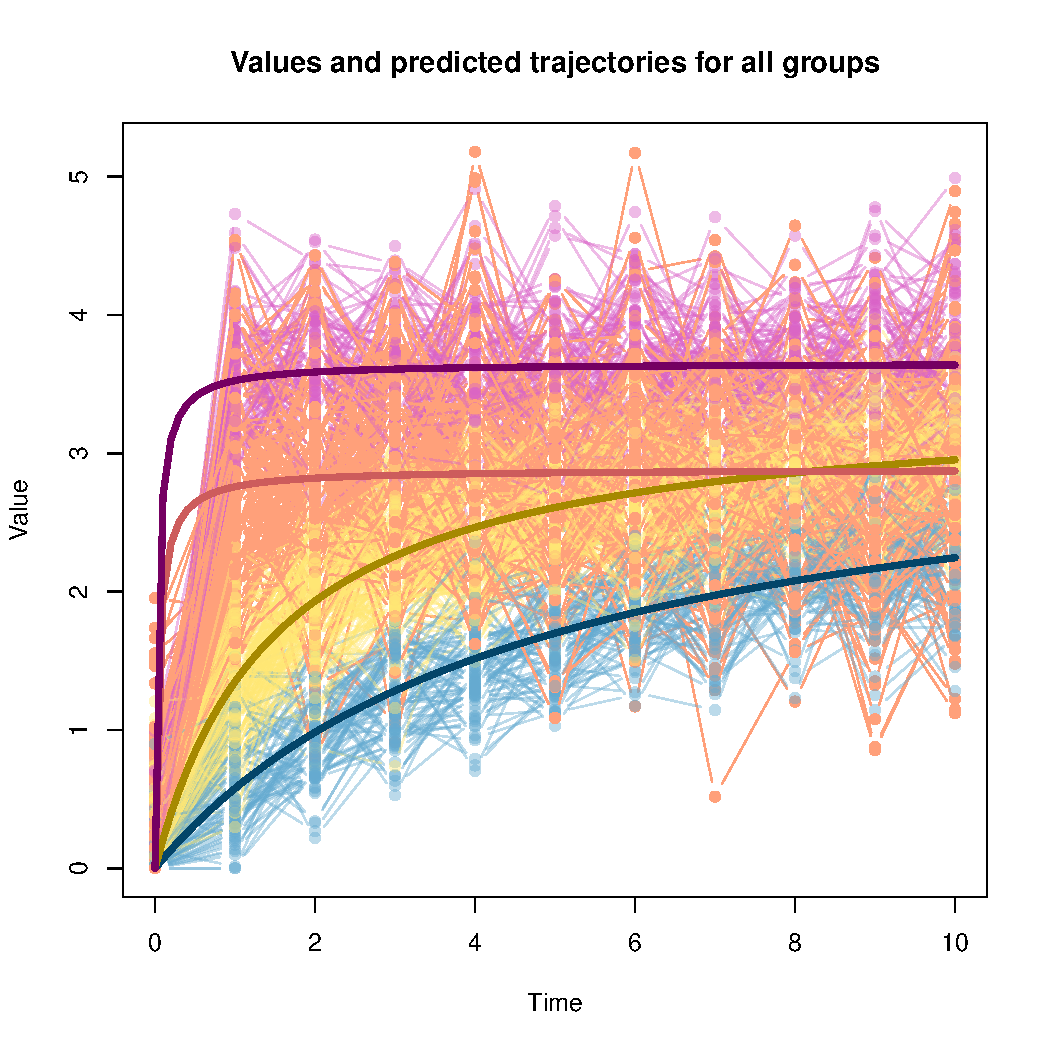
\includegraphics[width=\maxwidth]{figure/unnamed-chunk-75-1} 

\end{knitrout}
Here too we can add mean of each epoch to the plot.
\begin{knitrout}
\definecolor{shadecolor}{rgb}{0.969, 0.969, 0.969}\color{fgcolor}\begin{kframe}
\begin{alltt}
\hlkwd{plot}\hlstd{(solEM,} \hlkwc{Y}\hlstd{=data[,}\hlnum{2}\hlopt{:}\hlnum{12}\hlstd{],} \hlkwc{A}\hlstd{=data[,}\hlnum{13}\hlopt{:}\hlnum{23}\hlstd{],}\hlkwc{col} \hlstd{= vcol,} \hlkwc{mean} \hlstd{=} \hlnum{TRUE}\hlstd{)}
\end{alltt}
\end{kframe}
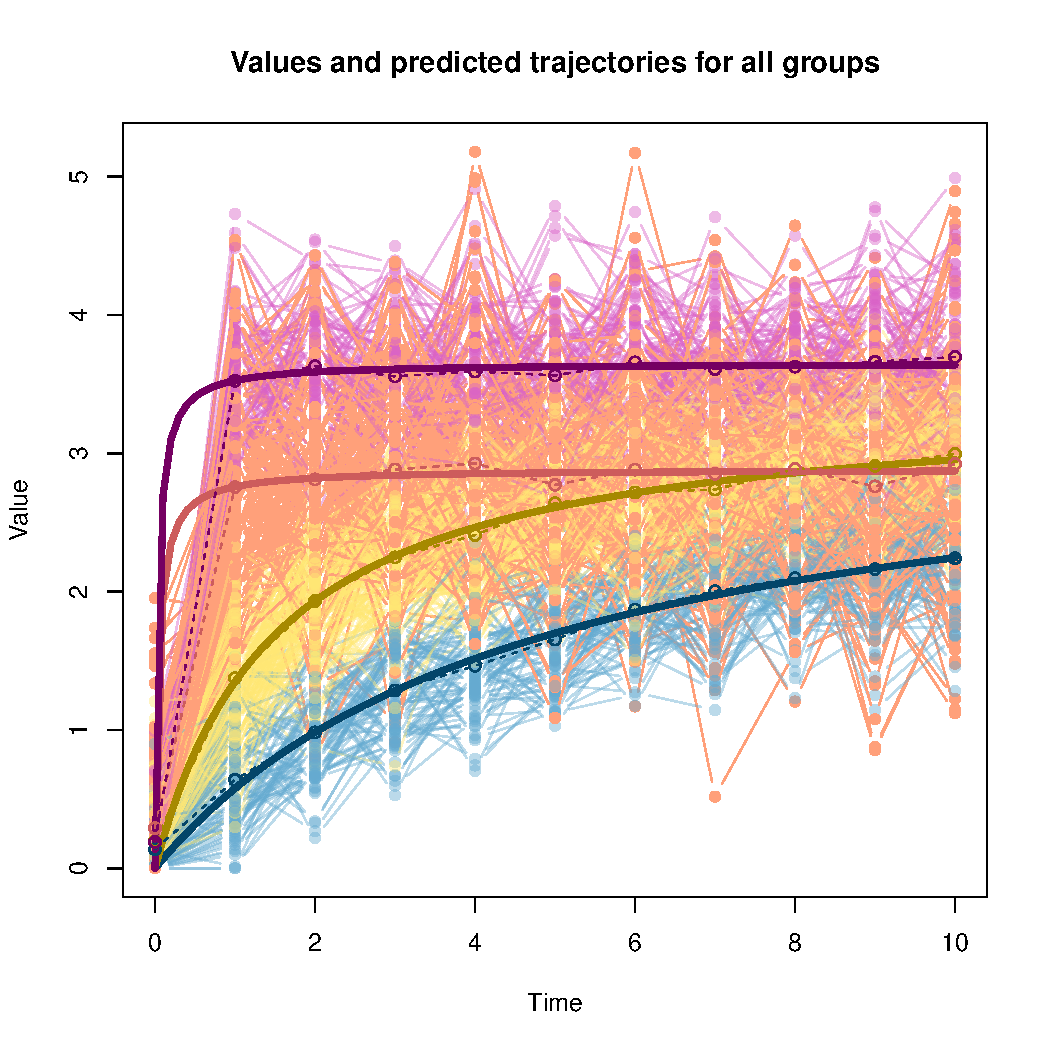
\includegraphics[width=\maxwidth]{figure/unnamed-chunk-76-1} 

\end{knitrout}

\section{Membership probability}

Sometimes it is util to find the membership probability of an individual for each group. The function \verb|GroupProb| do it. For each individual in the data it calculate the probability of membership of each group. The result is a matrix of real.\\

To illustrate this point we use the data and the results in the part page \pageref{probCens}.

\begin{knitrout}
\definecolor{shadecolor}{rgb}{0.969, 0.969, 0.969}\color{fgcolor}\begin{kframe}
\begin{alltt}
\hlstd{prob} \hlkwb{=} \hlkwd{GroupProb}\hlstd{(solLs,} \hlkwc{Y} \hlstd{=  data[,}\hlnum{2}\hlopt{:}\hlnum{11}\hlstd{],} \hlkwc{A} \hlstd{= data[,}\hlnum{12}\hlopt{:}\hlnum{21}\hlstd{])}
\hlkwd{head}\hlstd{(prob)}
\end{alltt}
\begin{verbatim}
##               Gr1          Gr2          Gr3
## [1,] 1.000000e+00 1.799408e-08 1.781027e-15
## [2,] 1.930888e-07 2.274434e-16 9.999998e-01
## [3,] 1.000000e+00 2.204867e-09 2.587772e-15
## [4,] 1.000000e+00 2.868289e-08 6.051662e-16
## [5,] 1.825766e-11 2.046285e-20 1.000000e+00
## [6,] 9.999999e-01 1.116069e-07 2.165143e-13
\end{verbatim}
\end{kframe}
\end{knitrout}


\end{document}
